\documentclass[12pt,onecolumn,a4paper,final,notitlepage]{report}

\usepackage[left=3.5cm,top=2.5cm,right=2.5cm,bottom=2.5cm,includehead,includefoot]{geometry}

\usepackage{footnote}
%\makesavenoteenv{tabular} 

\usepackage[noend]{algorithmic}
\usepackage{algorithm}
\usepackage{todonotes}
\usepackage[MeX]{polski}
\usepackage{url}
\usepackage{graphicx}
\usepackage{float}
\usepackage[justification=centering]{caption}
%\usepackage{subfloat}
\usepackage{subfig}
\usepackage{amsmath}
\usepackage{amssymb}
%\usepackage[countmax]{subfloat}
\usepackage{wrapfig}

%\usepackage{listingsutf8}
%\usepackage[latin1]{inputenc}
% Euro characters etc.
%\usepackage{textcomp}
% Works perfectly with latin1
\usepackage{listings}

\lstloadlanguages{XML,C++}
\usepackage{color}
\linespread{1.3}
\definecolor{light-gray}{gray}{0.85}
\graphicspath{{./grafika/}}
% kodowanie: latin2, utf8 lub cp1250
\usepackage[utf8]{inputenc}
\floatname{algorithm}{Algorytm}
\numberwithin{algorithm}{chapter}
\usepackage{longtable}
\usepackage{multicol}
\newcommand{\sgn}{\text{sgn}}

\usepackage{fancyhdr}
\setlength{\headheight}{15pt}
\pagestyle{fancy}
\lhead{\fancyplain{}{\nouppercase\leftmark}}
\chead{}
\rhead{}
\lfoot{}
\cfoot{\fancyplain{}{\thepage}}
\rfoot{}

\definecolor{orange}{rgb}{1.0,0.3,0.2}


\begin{document}
\begin{titlepage}
\linespread{1.1}
\hspace{0.4cm}
 \begin{minipage}{0.4\textwidth}
	\begin{flushleft} 
	
\includegraphics[scale=0.15]{./logo_pw_moje}
	\end{flushleft}
\end{minipage}
\begin{minipage}{0.4\textwidth}
	\begin{flushright} 
	
\includegraphics[scale=0.6]{./logo_weiti}
	\end{flushright}
\end{minipage}
\begin{flushleft}


\end{flushleft}
\vspace{0.1cm}
\begin{center}
{\textbf{\LARGE POLITECHNIKA WARSZAWSKA}}\\
\Large Wydział Elektroniki i Technik Informacyjnych\\
\Large Instytut Systemów Elektronicznych\\[2.5cm]
 \begin{minipage}{0.9\textwidth}
	\begin{center} 
	\Large
	Maciej Gąbka\\nr albumu: 198404
	\end{center}
\end{minipage}
\\[1.5cm]
{\Large Praca dyplomowa magisterska}\\
 \Huge Sterowanie robotem - zawodnikiem rozgrywek RoboCup\\[2.0cm]
\begin{flushleft} \large
\hspace{5.5cm}Praca wykonana pod kierunkiem \\ 
\hspace{5.5cm}prof. nzw. dr. hab. Jarosława Arabasa
\end{flushleft}
\vfill
% Bottom of the page
{\large Warszawa 2012}
\end{center}
\end{titlepage}

\input{./tex/streszczenie}

\tableofcontents

\chapter[Wstęp ]{Wstęp}
Szybki postęp technologiczny zapoczątkowany w XX wieku umożliwił rozwój nowych dziedzin nauki, między innymi robotyki. Obecnie maszyny mogą zastępować ludzi przy wykonywaniu wielu rozmaitych czynności.
Innowacyjne rozwiązania stwarzają jednak potrzebę opracowania wymagającego środowiska testowego. Jedną z takich inicjatyw, mających na celu wspieranie rozwoju i popularyzację robotyki, są rozgrywki
RoboCup. W obrębie przedsięwzięcia wyróżnionych jest kilka lig różniących się zasadami oraz typem robotów biorących udział w zawodach.
Głównym celem przyświecającym organizatorom jest stworzenie do 2050 roku drużyny robotów zdolnej wygrać z ówczesnymi mistrzami świata.
Liga RoboCup budzi zainteresowanie na całym świecie a prace z nią związane  są prowadzone w wielu środowiskach akademickich.
W Polsce nie została jeszcze stworzona drużyna, która wystartowałaby w tych rozgrywkach.
Rozwiązanie problemu stawia przed uczestnikami wyzwania konstrukcyjne oraz algorytmiczne. Niniejsza praca skupiona jest głównie na aspektach algorytmicznych. Omówiony zostanie problem sterowania
zawodnikiem, wyznaczania bezkolizyjnej ścieżki do celu oraz realizacji prostych zachowań niezbędnych podczas rozgrywek.
\section{Zakres pracy}
Niniejsza praca jest niejako kontynuacją działań podjętych podczas realizacji pracy inżynierskiej. Tematyka w niej poruszona dotyczy na wstępie samych rozgrywek RoboCup. Jak już napisano we 
wstępie przedsięwzięcie dotyczy głównie rozgrywek piłkarskich, w których udział biorą roboty. Jednak ze względu na dynamiczny rozwój samej robotyki uczestnicy projektu aaaa.
Obecnie podział jest następujący:
\begin{itemize}
	\item \emph{RoboCupSoccer}, czyli rozgrywki piłkarskie autonomicznych robotów,
	\item \emph{RoboCupRescue}, obejmujący działania robotów w sytuacjach kryzysowych, czy niebezpiecznych dla ludzi,
	\item \emph{RoboCup@Home}, skupiający się na robotyce mającej na celu pomaganie człowiekowi w codziennych czynnościach,
	\item \emph{RoboCupJunior} popularyzujący robotykę wśród młodzieży.
\end{itemize}

Same rozgrywki piłkarskie \emph{RoboCupSoccer} także są podzielone na kilka lig, tutaj głównym kryterium jest konstrukcja mechaniczna zawodników. Więcej informacji na ten temat zostanie zaprezentowanych w rozdziale
\ref{chap:robocup}. W ramach samej pracy skupiono się na lidze małych robotów (\emph{Small-size League}), ponieważ już wcześniej prowadzone były prace w tym kierunku na Wydziale Elektroniki i 
Technik Informacyjnych Politechniki Warszawskiej.

W dalszej części pracy opisano nowe testowe środowisko symulacyjne oraz wprowadzone poprawki modyfikujące działanie symulatora.
Z racji, iż wcześniejsze ekssperymenty prowadzono w środowisku \emph{Player/Stage/Gazebo} zdecydowano się na dalsze prace na tej platformie.
Opracowane zostały nowe modele zawodników wzorowane na rzeczywistych, holonomicznych
biorących udział w rozgrywkach. Przygotowano sterownik (element symulatora) umożliwiający: kontrolę nad prędkością robota (wyposażono go dodatkowo w regulator PID), prowadzenie piłki jak i oddawanie strzału.
 W stosunku do poprzednich prac zdecydowano się także na implementację oraz poddanie testom nowego algorytmu nawigacji.  Rozwiązanie to zostało przetestowane w takich samych warunkach 
jak poprzednie. Dokonano także analizy i porównania otrzymanych wyników. Zaprezentowano również inne, stosowane w robotyce, metody unikania kolizji. Jeden z nich został zaimplementowany w celu
rozwiązywania mniej złożonych zadań takich jak odjechanie od przeszkody w momencie wystąpienia kolizji.

W tekście przedstawiono jedno z podejść, powszechnie stosowanych do koordynacji i planowania działań zawodników (\mbox{\textit{STP - Skill Tactics Play}} \cite{stp}).
Zakłada ono planowanie zachowań drużyny na trzech poziomach. Każdy odnosi się do innej warstwy abstrakcji.
\begin{enumerate} 
  \item Najwyżej w hierarchii znajduje się poziom \texttt{Play}. Przez to pojęcie rozumiany jest plan gry dla całej drużyny uwzględniający koordynację
  poczynań pomiędzy zawodnikami. Plan również zakłada przydział zawodnika do określonej roli. W oryginalnym rozwiązaniu role przydzielane są dynamicznie w zależności od sytuacji na boisku.
  W obrębie danego planu zawodnik wykonuje swoją rolę (sekwencję kilku \textit{Tactic}) aż do momentu zakończenia danego planu lub wyznaczenia kolejnego.
  
  \item Przez \textit{Tactic} rozumiany jest plan działań w obrębie jednej roli. Taktyka ma na celu wykonanie przez robota pojedynczej złożonej akcji.
  Przykładem może być strzał na bramkę. Robot dostaje polecenie oddania strzału na bramkę, zatem plan jego poczynań ma doprowadzić
 do sytuacji, w której osiągnie on pozycję umożliwiającą oddanie strzału na bramkę z określonym powodzeniem.
 Plan na szczeblu pojedynczego robota jest wykonywany do momentu zmiany strategii gry całej drużyny (ponownego przydziału robotów do ról).
 Przykładowe \textit{Tactics}:
 \begin{itemize}
  \item strzał na bramkę,
  \item podanie piłki,
  \item odebranie podania,
  \item blokowanie innego robota,
  \item wyjście na pozycję,
  \item bronienie pozycji,
  \item dryblowanie z piłką.
 \end{itemize}

  Pojedyncza taktyka determinuje skończony automat stanów, w którym elementami są \texttt{Skills}. Wykonanie bieżącej taktyki sprowadza się do przechodzenia pomiędzy kolejnymi zachowaniami robota w obrębie
  danego automatu.
\newpage
  \item Najniżej w hierarchii znajduje się warstwa \textit{Skills}, odnosi się ono do konkretnych umiejętności robota, takich jak:
    \begin{itemize}
    \item przechwytywanie piłki,
    \item oddawanie strzału,
    \item doprowadzenie piłki do celu,
    \item przemieszczenie robota do celu,
    \item podążanie za innym robotem.
    \end{itemize}

  Na tym szczeblu nie występuje koordynacja w obrębie drużyny. W każdym kroku gry powinno być określone jakie zachowanie ma wykonywać robot. Z każdego \textit{Skill}, w każdym momencie określone musi być przejście
  do nowego zadania bądź kontynuowanie tego samego zadania. Przykładowo jeśli zlecimy robotowi przemieszczenie się z piłką do celu a piłka 
  odskoczy robotowi, to powinien do niej podjechać, przechwycić ją, a następnie ponownie prowadzić do zadanego celu (należy jednak cały czas pamiętać, że jeśli nastąpi dobra okazja do strzału
na bramkę, robot powinien ją wykorzystać).
\end{enumerate}

 W ramach pracy w pełni zrealizowane zostały dwie warstwy z oryginalnej hierarchii opisanej powyżej (\textit{Skills} oraz \textit{Tactics}). Aplikację projektowano w taki sposób, aby pozostawić miejsce
 na pełną implementację warstwy \textit{Play}, którą zrealizowano jedynie w stopniu niezbędnym do przeprowadzenia eksperymentów.
Użyteczność algorytmu sprawdzono podczas przeprowadzonych eksperymentów, wzorowanych na rzeczywistych zadaniach eliminacyjnych stosowanych w rozgrywkach RoboCup w ostatnich latach.

\section{Cel pracy}
Za główny cel niniejszej pracy postawiono stworzenie oprogramowania umożliwiającego wykonywanie podstawowych elementów gry w piłkę nożną przez roboty. W tym celu posłużono się architekturą STP. Aby jednak zrealizować to zadanie konieczne było
stworzenie środowiska symulacyjnego, umożliwiającego modelowanie rozgrywki \emph{Small-size League}. Przy opracowywaniu modelu środowiska starano się w jak największym stopniu odzwierciedlić realia
ligi \emph{Small-size League}. Po drugie środowisko symulacyjne miało być na tyle elastyczne, aby w przyszłości umożliwiało testowanie różnorodnych rozwiązań sterowania drużyną.
Zachowano schemat przepływu informacji z pracy inżynierskiej, który zamieszczono na rysunku \ref{fig:przeplyw_sterowania}. Stosowany w rozgrywkach \emph{Small-size League} \textit{videoserver} został
ujęty w osobną warstwę  aplikacji komunikująca się bezpośrednio z symulatorem. Osobną warstwę stanowi także część aplikacji odpowiedzialna za sterowanie robotem.
\begin{figure}[H]
\centering
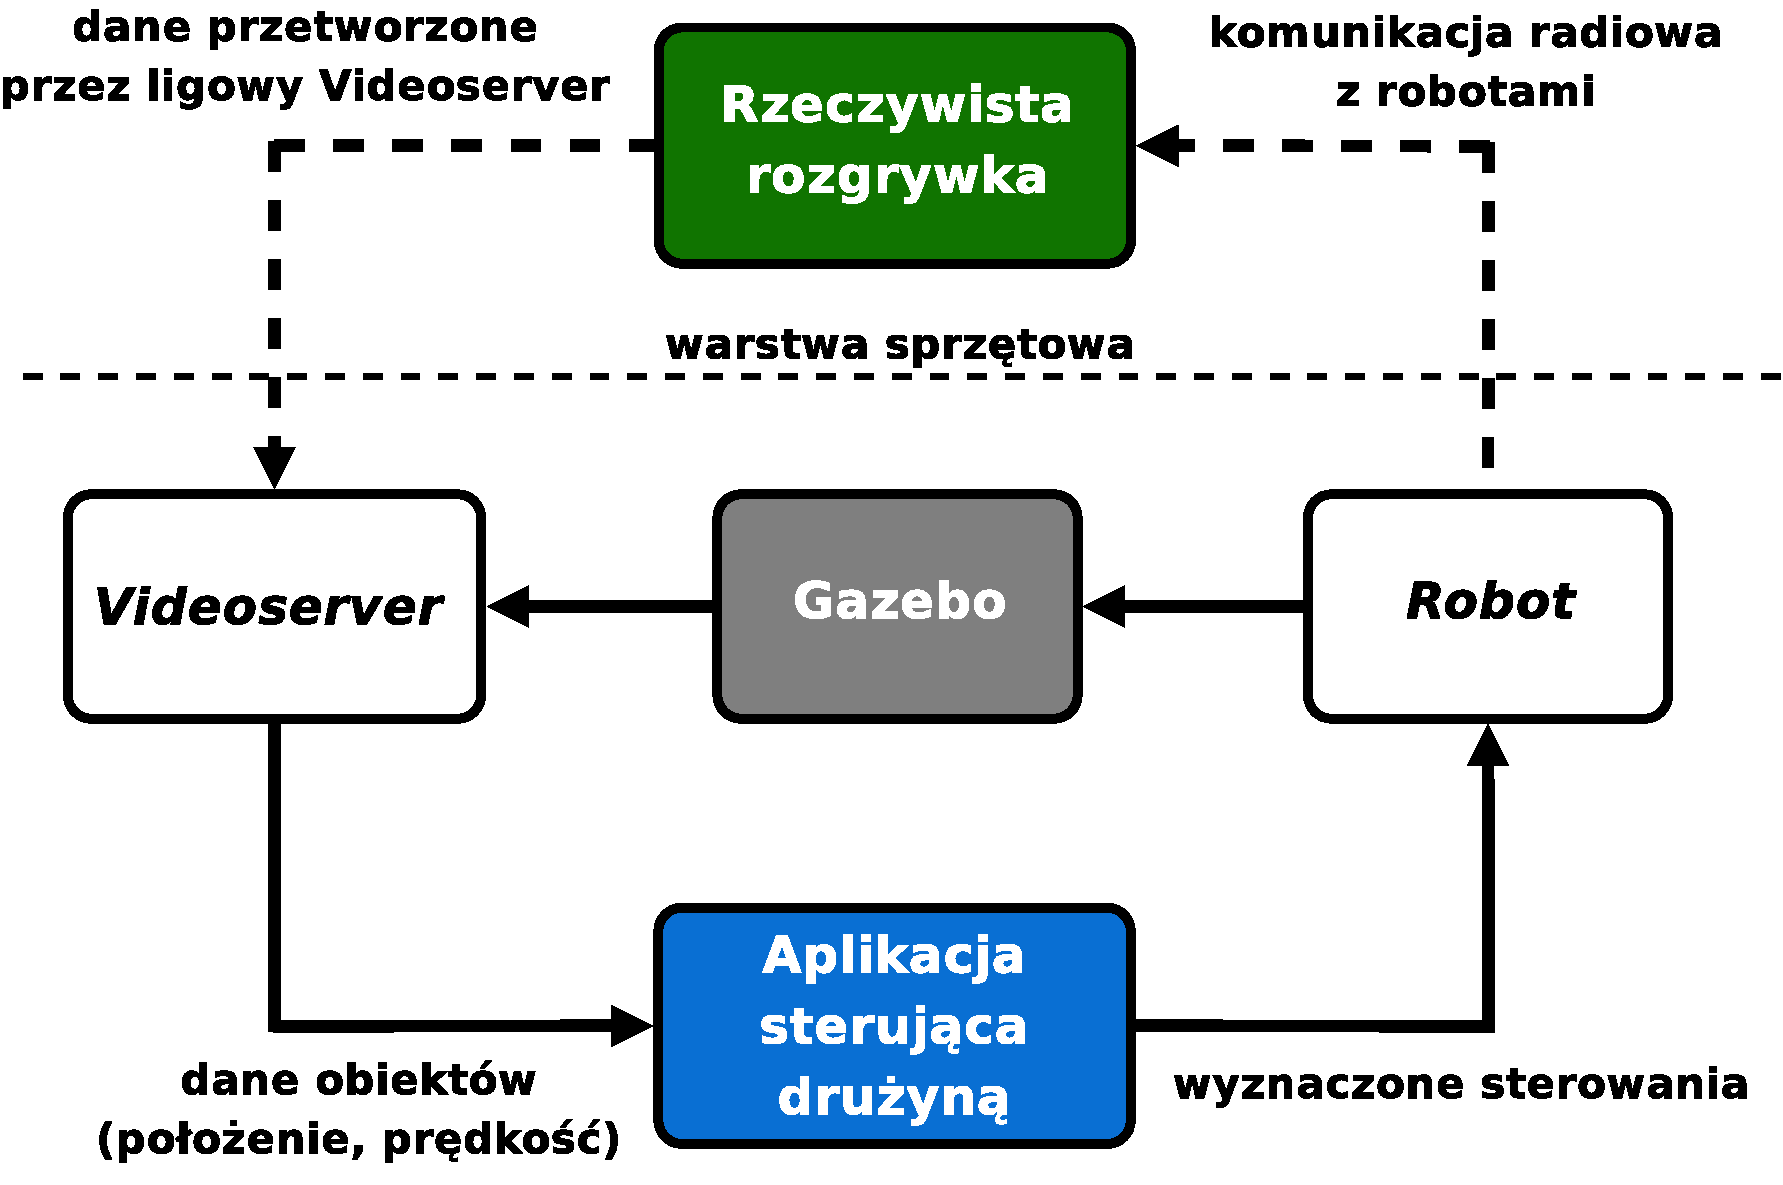
\includegraphics[scale=0.38]{./zalozenia/przeplyw_sterowania.png}
\caption{Komunikacja pomiędzy warstwami aplikacji.} \label{fig:przeplyw_sterowania}
\end{figure}
Główną motywacją takiej architektury było umożliwienie prostego przystosowania aplikacji do sterowania rzeczywistym robotem pobierającym dane z zewnętrznego serwera. 
Ponieważ w rozgrywkach biorą udział roboty holonomiczne, zdecydowano się na odejście od modelu robota o napędzie różnicowym stosowanego w pracy inżynierskiej. Opracowano zatem nowy model wzorowany na rzeczywistych
zawodnikach.
Kolejnym celem pracy, wynikającym bezpośrednio ze zmiany modelu robota, było zaimplementowanie i przetestowanie algorytmu nawigacji w dynamicznym środowisku. Zdecydowano się na algorytm RRT,
postanowiono także porównać jego skuteczność z wcześniej stosowanym CVM.



\chapter{Liga Robocup}

\begin{abstract}
 Rozdział zostanie w całości poświęcony opisowi projektu Robocup.
Więcej informacji na ten temat należy poszukiwać na oficjalnej stronie projektu \url{http://www.robocup.org}
Zaprezentowana zostanie pokrótce historia samej idei projektu, jej rozwój oraz  poszczególne ligi wchodzące w skład całego projektu.
Głównie zostanie omówiona \emph{Small-size League}, ze szczególnym uwzględnieniem modelu robote i ograniczeń z tym związanych.
\end{abstract}


	\section{Omówienie projektu robocup}
		\subsection{Krótki opis genezy}
		\subsection{Podział na ligi robotów}
		\begin{itemize}
			\item Najstarsza z lig, liga symulacyjna
			\item Omówienie ligi \emph{Small-size League}
			\item Omówienie ligi \emph{Middle-size League}
			\item Omówienie ligi \emph{Standard Platform League }
			\item Omówienie ligi \emph{Humanoid League}
			\item \emph{RoboCupRescue} - wykorzystanie dorobku robotyki w służbie ludziom
		\end{itemize}


	\section{Specyfika ligi small-size (F180)}
	W paragrafie zostaną ujęte i dokładnie opisane zasady ligi(dzieki temu można będzie wyjaśnić rodzaj architektury zastosowanej w
	aplikacji sterującej). Po krótce zostanie przedstawiony model robota wykorzystywany w lidze ze szczególnym uwzględnieniem 
	elementów służących do podawania oraz prowadzenia piłki. Dodatkowo zostanie zaprezentowany schemat komunikacji wykorzystywany w lidze.
	\subsection{Zasady}
		\begin{itemize}
		 \item zaprezentowanie wymogów technicznych dotyczących :
			\begin{itemize}
 			\item{wymiarów robota}
			\item{wymiarów boiska}
			\item{liczby robotów}
			\item{sposobów prowadzenia piłki}  
			\end{itemize}
 		\item omówienie podstawowych zasad takich jak:
			\begin{itemize}
			 \item sygnalizowanie przewinień
			 \item rola arbitra podczas rozgrywki
			\end{itemize}
		\end{itemize}


	\subsection{Budowa robota}
		\begin{itemize}
	 	\item Zaprezentowanie konstrukcji robotów z ligi \emph{small-size}
			\begin{itemize}
			\item omówienie bazy jezdnej
			\item zaprezentowanie urządzenia umożliwiającego prowadzenie piłki
 			\item rola znaczników umieszczonych na konstrukcji mechanicznej robota
			\item dostępne czujniki (określone przez regulamin)
			\end{itemize}
		\end{itemize}


\chapter[Player/Stage/Gazebo ]{Player/Stage/Gazebo \label{chap:gazebo}}
\chaptermark{Player/Stage/Gazebo}
	Symulator \mbox{\texttt{Player/Stage/Gazebo}} został już opisany w pracy inżynierskiej \cite{inzynierka} jednak z uwagi na jego ważną rolę i zmiany jakie zdecydowano się wprowadzić w symulowanym
	środowisku podczas rozwijania aplikiacji zdecydowano się na krótkie przypomnienie koncepcji projektu.

	\section{Koncepcja}
	Oprogramowanie składa się z trzech niezależnych aplikacji \textit{Player}, \textit{Stage} oraz \textit{Gazebo}.
	\textit{Gazebo} oraz \textit{Stage} są środowiskami symulacyjnymi. Z tą różnicą, że \textit{Stage} jest środowiskiem dwuwymiarowym, dedykowanym do symulowanie dużych populacji robotów
	mobilnych. Natomiast \textit{Gazebo} zapewnia pełną trójwymiarową symulację, uwzględniając również oddziaływania fizyczne pomiędzy stosowanymi obiektami.
	W trakcie realizacji niniejszej pracy wydana została pierwsza stabilna wersja oprogramowanie dostępna pod adresem \url{http://gazebosim.org}.
	Wcześniej wszelkie dane dotyczące wszystkich aplikacji wchodzących w skład projektu dostępne były na stronie \url{http://playerstage.sourceforge.net}. Z uwagi na trudności związane z adaptacją
	symulatora zdecydowano się na kontynuację prac na wersji pobranej ze starego repozytorium.
	Ostatnia aplikacja wchodząca w skład projektu, czyli \textit{Player} jest serwerem sieciowym służącym do sterowania rzeczysiwtymi robotami. Dostarcza prosty interfejs, wspierający komunikację z wieloma 
	typami powszechnie stosowanych czujników i aktuatorów.
	Oprogramowanie jest kompatybilne z systamami Linux, Solaris, *BSD oraz Mac OSX.
	W niniejszej pracy zdecydowano się na wykorzystanie jedynie symulatora \textit{Gazebo}.

	\section{Architektura symulatora}
	\begin{figure}[!b]
	\centering
	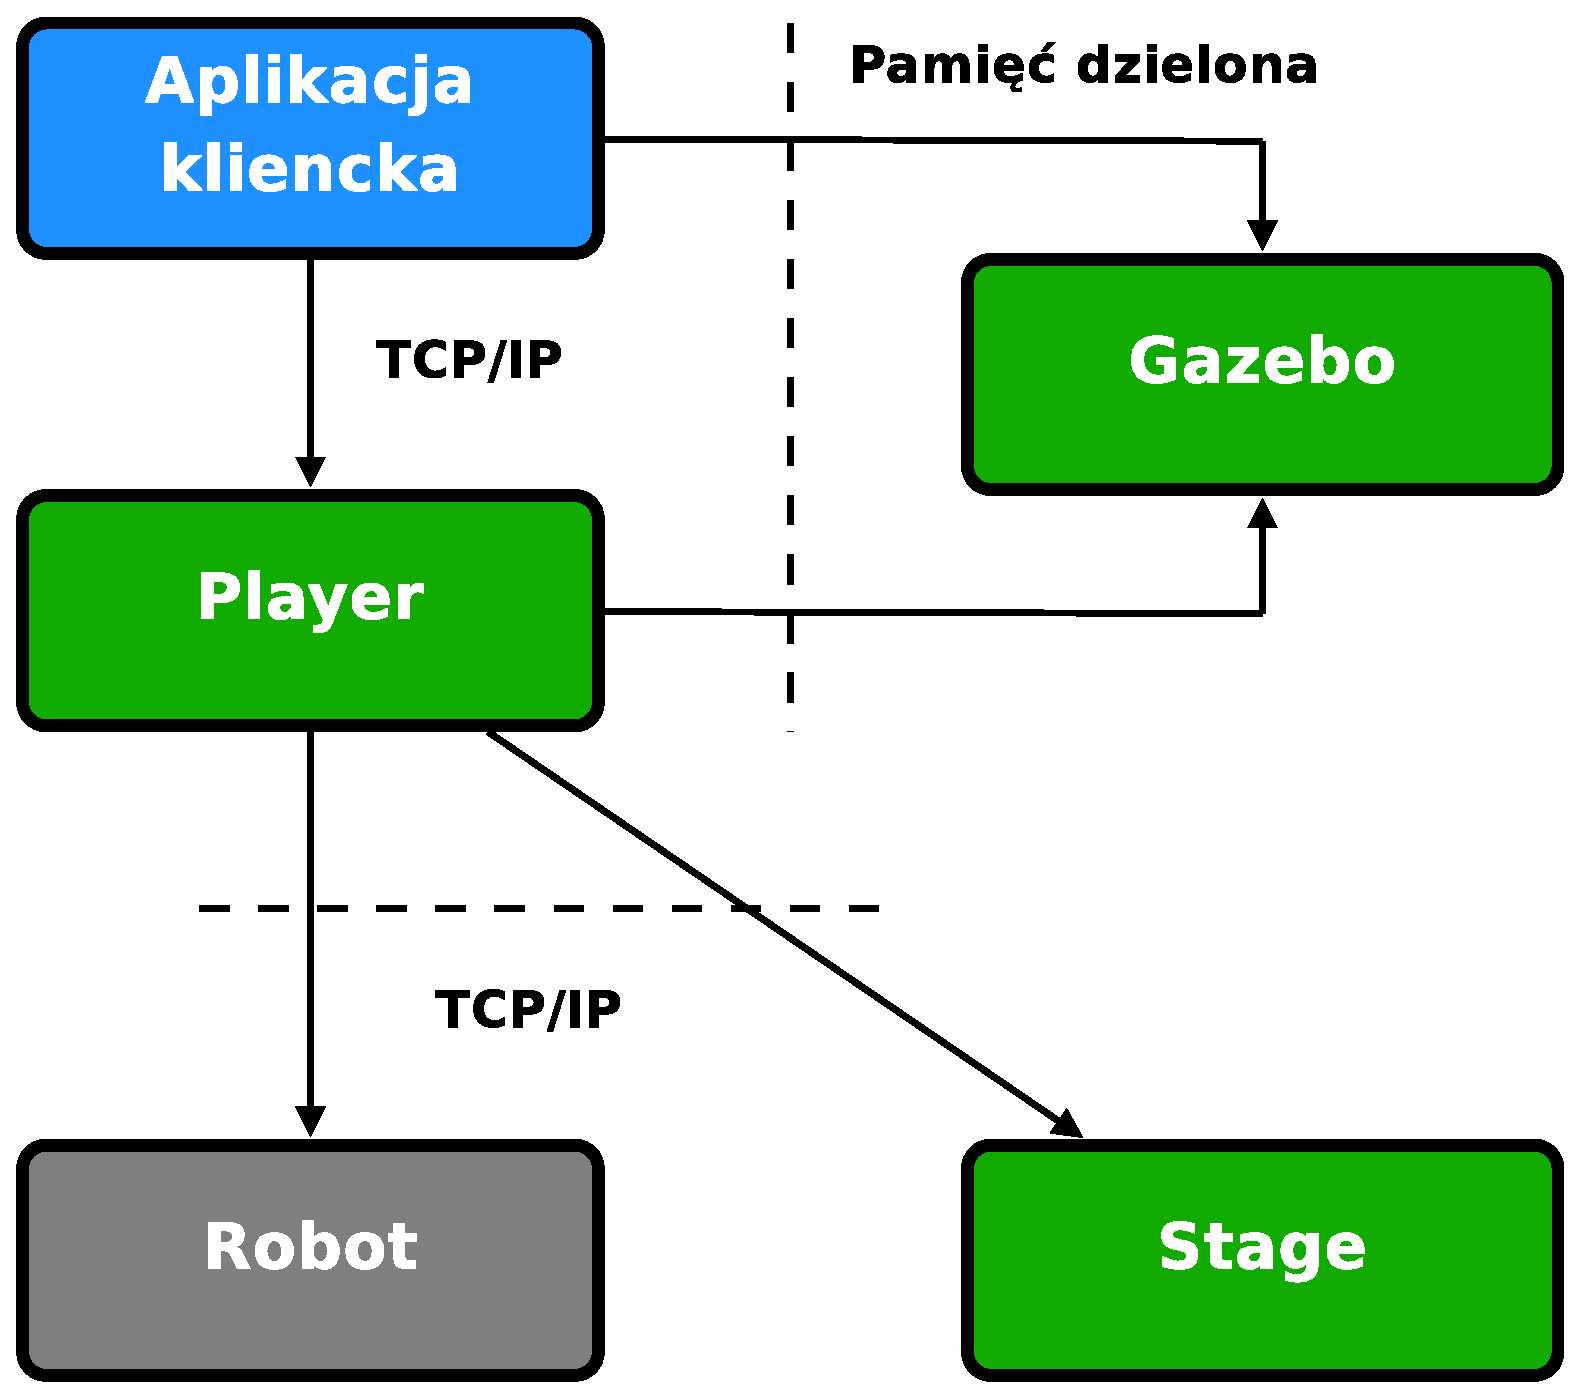
\includegraphics[scale=0.3]{./gazebo/architektura}
	\caption{Schemat komunikacji w środowisku \textit{Player/Stage/Gazebo} \label{fig:arch}}
	\end{figure}
	
	Wymiana informacji pomiędzy elementami środowiska symulacyjnego \textit{Player/Stage/Gazebo} została przedstawiona na 
	rysunku~\ref{fig:arch}.
	Po zapoznaniu się z nim , można lepiej zrozumieć rolę programu \textit{Player}. Pełni on funckję pośrednika pomiędzy aplikacją klienta, stworzona przez użytkownika
	a rzeczywistym robotem lub symulatorami modelującymi jego zachowanie w tym przypadku (\textit{Stage} lub \textit{Gazebo}). 
	Komunikacja pomiędzy \textit{Player-em}, robotem oraz aplikacją kliencką realizowana jest za pomocą protokołu TCP/IP.
	Dzięki takiej architekturze z punktu widzenia klienta nie istotne jest, czy interfejsy udostępnione przez \textit{Player-a} sterują rzeczywistym robotem, czy symulowanym odpowiednikiem.
	
	Z samym symulatorem, zarówno \textit{Stage} jak i \textit{Gazebo} można komunikować się poprzez pamięć współdzieloną (rysunek \ref{fig:wybrana_arch}), bez wykorzystywania aplikacji \textit{Player}. Rozwiązanie to jest 
	preferowane w sytuacji gdy korzystanie z \textit{Playera} nie jest uzasadnione, lub kiedy użytkownik dokonał modyfikacji działania symulatora, których nie implementuje \textit{Player}. 
	Aplikacja \textit{Gazebo} udostepnia w tym celu  bibliotekę \textit{libgazebo}, dostarczającą zestaw funkcji do komunikacji.
	\begin{figure}[h]
	\centering
	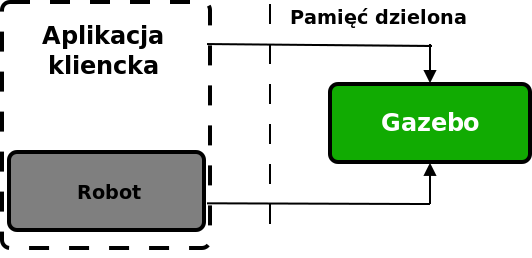
\includegraphics[scale=0.3]{./gazebo/wybrana_architektura}
	\caption{Zrealizowany schemat komunikacji w środowisku \textit{Player/Stage/Gazebo} \label{fig:wybrana_arch}}
	\end{figure}
	Z tego właśnie rozwiązania zdecydowano się skorzystać w niniejszej pracy. Po pierwsze, dlatego iż zmniejsza to nakład niezbędnych prac, po drugie iż nie posiadano rzeczywistego modelu
	zawodnika. Wprowadzone poprawki podczas opracowania środowiska testowego oraz przygotowanie własnego sterownika robota, także nasunęły to rozwiązanie.

	Podsumowując, struktura pakietu oprogramowania \mbox{\textit{Player/Stage/Gazebo}} umożliwia tworzenie aplikacji sterujących robotami w sposób,
	który zapewnia przenośność stworzonych programów i ich działanie zarówno na symulatorach robotów, jaki i na rzeczywistych obiektach.
	
 	\subsection{Gazebo}
 	
 	Symulator \textit{Gazebo} jak wynika z wcześniejszego tekstu, umożliwia symulację grup robotów mobilnych. Symulowane
 	środowisko jest w pełni trójwymiarowe, uwzględniona jest dynamika brył oraz obliczane rzeczywiste oddziaływania między komponentami symulowanego świata.
	Okupione jest to oczywiście większym niż w przypadku \textit{Stage} zużyciem mocy obliczeniowej, dlatego symulowane populacje robotów nie powinny być zby liczne.
 	 	
 	Trzy najistotniejsze kompnenty wykorzystywane przez rogram \textit{Gazebo} to:
 	\begin{itemize}
 	 \item ODE\footnote{Open Dynamics Engine, \url{http://www.ode.org}}, biblioteka  odpowiadająca za symulację
 	 	zależności fizycznych pomiędzy bryłami oraz detekcję kolizji,
 	 \item OGRE\footnote{Object-Oriented Graphics Rendering Engine, \url{http://www.ogre3d.org/}}, 
		silnik graficzny umożliwiający tworzenie wspomaganej sprzętowo grafiki 3D,
 	 \item FLTK\footnote{Fast Light Toolkit, \url{http://www.fltk.org/}}, biblioteka dostarczająca 
		przenośny interfejs użytkownika dla \textit{Gazebo}.
 	\end{itemize}

	W \textit{Gazebo} możliwe jest symulowanie standardowych sensorów stosowanych w robotyce (m.in. czujniki odległości, kamery, GPS). Symulator wyposażony jest w gotowe modele 
	popularnych robotów (jak np. \textit{Pioneer2DX}, \textit{Pioneer 2AT} oraz \textit{SegwayRMP}).
	Dozwolone jest także tworzenie własnych modeli
	Pozwala ponadto na tworzenie własnych modeli, z możliwością konfigurowania ich właściwości fizycznych (takich jak np. masa, współczynnik tarcia, sztywność).
	Dzieki temu środowisko może w dużym stopniu odzwierciedlać rzeczywistość. Modele można wyposażyć w jeden ze zdefiniowanych kotrolerów umożliwiających sterowanie (zadawanie prędkości, 
	czy odczyt danych z sensorów) lub opracować własny.
	\begin{figure}[!t]
	\centering
	\label{fig:gazebo}
	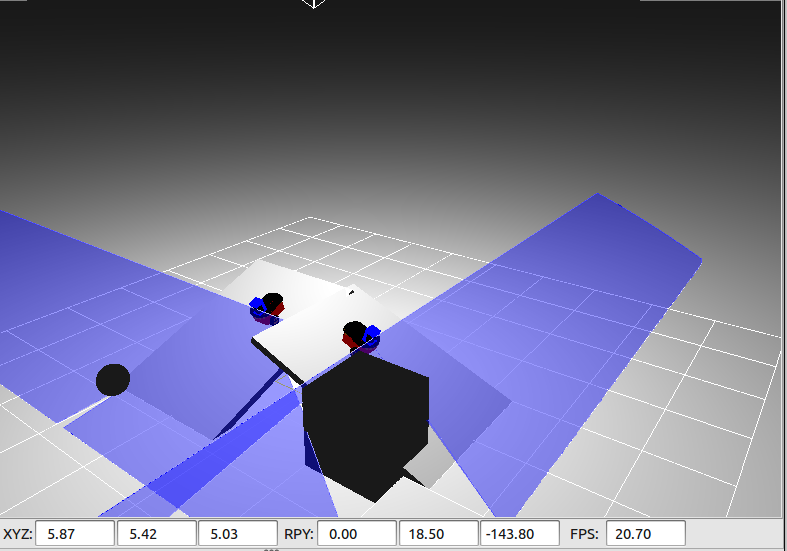
\includegraphics[scale=0.42]{./gazebo/gazebo_screen}
	\caption{\textit{Gazebo} -- okno główne (wersja 0.10)}
	\end{figure}

	\section{Modelowanie obiektów w Gazebo}
	Tworzenie symulowanego środowiska w \textit{Gazebo} polega na opracowaniu opisu świata w pliku z rozszerzeniem \textit{.world} za pomocą języka XML. W pliku powinny zostać zamieszczone parametry
	określające przebieg symulacji oraz informacje o występujących w danym świecie modelach.
	
	\subsection{Zasady modelowania w Gazebo 0.10}
	Forma pliku \textit{.world} zawierającego opis symulowanego środowiska daje użytkownikowi możliwość konfiguracji wielu kluczowych elementów takich jak: konfiguracja graficznego interfejsu użytkownika,
	zmianę sposobu renderowania sceny, wybór metody detekcji kolizji, zmianę wartości globalnych parametrów symulacji (m.in krok pracy symulatora). Elementy przykładowego pliku \textit{.world} zostały zaprezentowane na listingach poniżej.
	%\small
	%\lstset{language=XML,  basicstyle=\ttfamily\footnotesize,
	\lstset{language=XML,  basicstyle=\ttfamily\scriptsize, 
	commentstyle={}, xleftmargin=20pt, numbers=left, numberstyle=\footnotesize,
	caption={},
	backgroundcolor=\color{light-gray},
	frame=single,
	breaklines=true}
	\begin{lstlisting}[name=gazebo_simple_world]
	<?xml version="1.0"?>
	<gazebo:world>
	\end{lstlisting}
	Bardzo istotnym elementem jest konfiguracja fizyki (ODE), interfejs umożliwia konfigurację globalnych parametrów takich jak:
	\begin{lstlisting}[name=gazebo_simple_world]
	<physics:ode>
		<stepTime>0.001</stepTime>
		<gravity>0 0 -9.8</gravity>		
		<erp>0.8</erp>
		<cfm>0.05</cfm>
		<stepType>quick</stepType>
		<stepIters>25</stepIters>
		<stepW>1.4</stepW>
		<contactSurfaceLayer>0.007</contactSurfaceLayer>
		<contactMaxCorrectingVel>100</contactMaxCorrectingVel>
	 </physics:ode>
	\end{lstlisting}
	\lstset{language=XML,  basicstyle=\ttfamily\footnotesize, 
	commentstyle={}, xleftmargin=20pt, numbers=left, numberstyle=\footnotesize,
	caption={},
	backgroundcolor=\color{light-gray},
	frame=single,
	breaklines=true}
	Znaczenie poszczególnych parametrów jest następujące:
	\begin {enumerate}
	 \item \texttt{stepTime} jest wyrażony w sekundach i określa czas pomiędzy kolejnymi aktualizacjami silnika \texttt{ODE},
	 \item \texttt{gravity} jest wektorem określającym siłę grawitacji,
	 \item \texttt{erp} rozwija się na \textit{error reduction parameter}, przyjmuje on wartości z przedziału od $0$ do $1$ i jest odpowiedzialny za redukcję błędów w połączeniach pomiędzy bryłami
	  (problematyka zostanie szerzej poruszona na stronie \pageref{fig:joints}); \texttt{erp} ustawione na $0$ powoduje, że żadna dodatkowa siła nie jest przykładana do danej bryły, natomiast wartość $1$
	 powoduje, że wszytskie błędy połączeń zostaną naprawione w kolejnym kroku symulatora,
	 \item \texttt{cfm} jest skrótem od \textit{constraint force mixing} i odpowiada za sztywność ograniczeń występujacych w kolizjach między bryłami, gdy wartość jest równa $0$ ograniczenie wynikające z fizyki
nie może zostać złamane, ustawienie parametru na wartość dodatnią powoduje, że ograniczenie staje się ``miękkie'', sprężyste,
	  
	 \item \texttt{stepType} odpowiada za rodzaj używanej funkcji z \texttt{ODE} do detekcji kolizji, użytkownik może dokonać wybrou jednej z dwóch wartości:
	      \begin{itemize}
	       \item \textit{world}, używana jest wtedy funkcja \texttt{dWorldStep}, operująca na macierzy zawierającej wszystkie ograniczenia, złożoność obliczeniowa tej metody wynosi $m^3$, natomiast pamięciowa
jest rzędu $m^2$, gdzie $m$ określa ilość wierszy (ograniczeń) analizowanej macierzy,
	       \item \textit{quick}, do detekcji kolizji stosowana jest metoda iteracyjna, w literaturze nazywana \texttt{SOR - Successive over-relaxation} należąca do rodziny metod Gaussa–Seidela, jej złożoność obliczeniowa jest rzędu $m*N$,
		a pamięciowa $m$, gdzie $m$ ma znaczenie jak wyżej,
		natomiast $N$ jest liczbą iteracji; dla dużych systemów metoda jest dużo bardziej wydajna jednak mniej dokładna, mogą także występować problemy z jej stabilnością; najprostszą metodą na poprawę stabilności
		jest zwiększanie \texttt{cfm}, 
	      \end{itemize}
	 \item \texttt{stepIters} - ilość iteracji, gdy do detekcji kolizji wybrano metodę \textit{quick},
	 \item \texttt{stepW} określa czas relaksacji metody Gaussa–Seidela, 
	 \item \texttt{contactSurfaceLayer} określa głębokość na jaką może wnikać bryła w podłoże, ustawienie parametru na małą wartość dodatnią zapobiega jitterowi w momencie, gdy ograniczenia są nieustannie tworzone
	  i zrywane (na przykład podczas ruchu koła po podłożu),
	 \item \texttt{contactMaxCorrectingVel} jest maksymalną korektą prędkości jaka może wynikać z utworzonych tymczasowo kontaktów; domyślnie parametr przyjmuje nieskończoną wartość zmniejszanie jego
	   wartości może zapobiec tworzeniu się zagnieżdzonych kontaktów. 
	\end {enumerate}
	Warto wspomnieć, że niektóre parametry można zmieniać dla poszczególnych modeli lub połączeń \textit{joints}.\newline
	Ustawienia interfejsu: typ (dostępne tylko \textit{fltk}), rozmiaru okna i jego pozycja początkowej:
\begin{lstlisting} [name=gazebo_simple_world]
    <rendering:gui>
        <type>fltk</type>
        <size>640 480</size>
        <pos>0 0</pos>
    </rendering:gui>
\end{lstlisting}
	Określenie parametrów renderowanej sceny: techniki cieniowania, tekstury pokrywającej niebo (dostępne inne opcje, jak np. rodzaje oświetlenia, dodawanie mgły itp.):
\begin{lstlisting} [name=gazebo_simple_world]
    <rendering:ogre>
        <shadowTechnique>stencilAdditive</shadowTechnique>
        <sky>
              <material>Gazebo/CloudySky</material>
        </sky>
    </rendering:ogre>
</gazebo:world>
\end{lstlisting}

	Do tak stworzonego pliku z opisem świata należy następnie dodać modele.  Dodany obiekt musi zawierać co najmniej jeden element \textit{body}, który jest złożony z elementów \textit{geoms}. Sekcja opisująca przykładowy model piłki mogłaby wyglądać następująco:
	\begin{figure}[H]
	\centering
	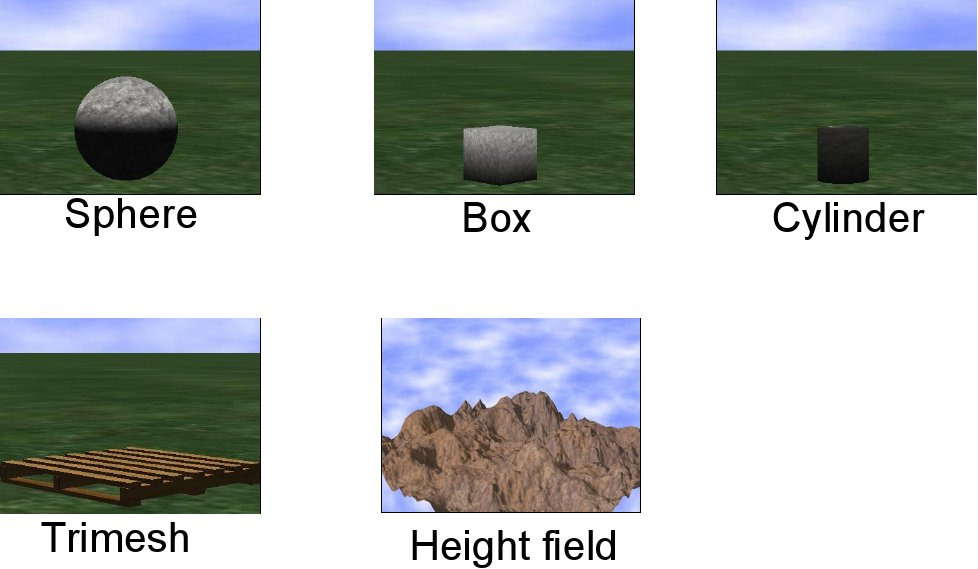
\includegraphics[scale=0.35]{./gazebo/geoms}
	\caption[Dostępne typy \textit{geoms}]
		{\label{fig:geoms}Dostępne typy \textit{geoms} -- Gazebo 0.10 (źródło:~\cite{gazebo_experts})}
	\end{figure}
	
	\lstset{language=XML,  basicstyle=\ttfamily\footnotesize, 
	commentstyle={}, xleftmargin=20pt, numbers=left, numberstyle=\footnotesize,
	caption={},
	backgroundcolor=\color{light-gray},
	frame=single,
	breaklines=true}
\begin{lstlisting}[name=gazebo_przyklad_pilka]
<model:physical name="ball">
    <static>false</static>
\end{lstlisting}
Na wstępie deklarowany jest model, którego parametr \textit{static} ustawiono na \textit{false}, co oznacza, że będzie on brał udział
w symulacji fizycznej i może oddziaływać z innymi obiektami. Następnie należy zadeklarować ``ciało'' tworzonego obiektu:
\begin{lstlisting}[name=gazebo_przyklad_pilka]
    <body:sphere name = "ball_body">	
\end{lstlisting}
Wewnątrz \textit{body}, które jest odpowiedzialne za dynamikę obiektu, należy umieścić elementy opisujące kształt obiektu (pozwalające tym samym na detekcję kolizji) -- w tym przypadku zdefiniowano kulę o wymiarach i masie odpowiadającej piłce do golfa:
\begin{lstlisting}[name=gazebo_przyklad_pilka]
	<geom:sphere name = "ball_geom">
		<xyz>0 0 0.01</xyz>
		<rpy>0 0 0 </rpy>
		<size>0.02</size>
		<mass>0.045</mass>
\end{lstlisting}
Sekcja \textit{visual} bloku \textit{geom} pozwala na przypisanie obiektowi wyglądu -- może to być figura o dowolnym kształcie (stworzona np. w programie do grafiki 3D) i wybranej przez projektanta teksturze lub kolorze:
\begin{lstlisting}[name=gazebo_przyklad_pilka]
		<visual>	
			<scale>0.02 0.02 0.02</scale>
			<size>0.02</size>
			<mesh>unit_sphere</mesh>
			<material>Gazebo/Orange</material>
		</visual>
	</geom:sphere>				
    </body:sphere>
</model:physical>
\end{lstlisting}	


	
	\subsubsection{Połączenia pomiędzy bryłami }
	Tworząc modele, można korzystać z trzech podstawowych brył (kula, walec, prostopadłościan), a także z siatek \textit{trimesh} oraz elementów \textit{height field} (stworzonych do generowana terenu -- por. rys. \ref{fig:geoms})).
	Żeby zamodelować robota, należy jeszcze stworzone bryły odpowiednio ze sobą powiązać. Do tego służą elementy typu \textit{joint}, którymi można łączyć komponenty \textit{body} (modelujące np. koła i podwozie robota).
	Stopnie swobody połączenia zależą od wybranego typu wiązania \textit{joint} (dostępne typy przedstawiono na rys. \ref{fig:joints}). Obiekty połączone wiązaniem tworzą parę kinematyczną.
	\textit{Gazebo} umożliwia nadawanie tak połączonym bryłom prędkości obrotowych względem siebie, co pozwala na modelowanie ruchomych elementów robotów.
	\begin{figure}[H]
	\centering
	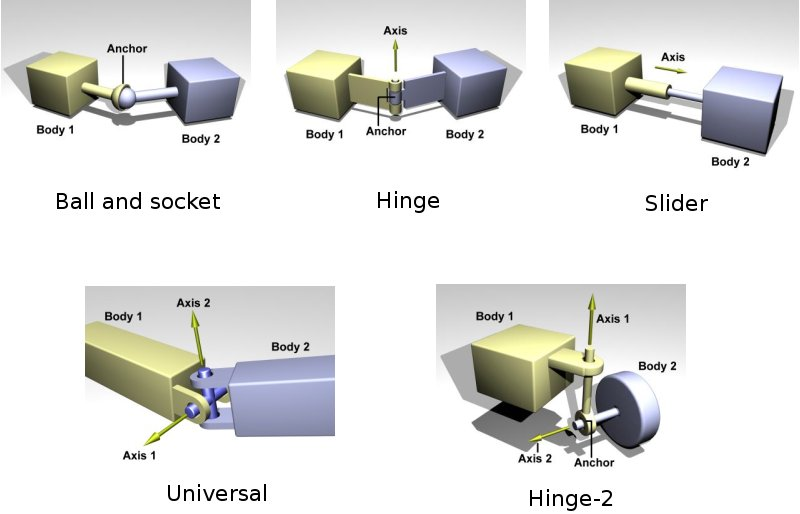
\includegraphics[scale=0.43]{./gazebo/joints}
	\caption{Typy połączeń \textit{joints} (Źródło: dokumentacja ODE) \label{fig:joints}}
	\end{figure}
	Jak wspomniano wcześniej, w czasie realizowanej symulacji połączenia pomiędzy bryłami moga ulec wypaczeniu, na skutek sił działających na model. Może to być tarcie,
	siła powodująca obrót bryły czy siły działające na model podczas kolizji. Sytacje taką przedstawiono na rysunku \ref{fig:bad_joint}.
	\begin{figure}[H]
	\centering
	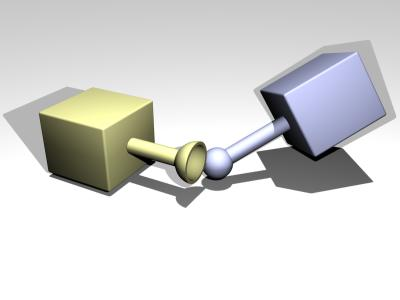
\includegraphics[scale=0.43]{./gazebo/bad_joint}
	\caption{Zepsute połączenie (\textit{joints}) (Źródło: dokumentacja ODE) \label{fig:bad_joint}}
	\end{figure}
	Błędy tego typu można redukować za pomocą parametru \texttt{erp} ustawianego globalnie lub dla każdego z połączeń indywidualnie.
	\subsubsection{Sterowniki modeli }
	Sterowanie zaprojektowanym modelem jest możliwe po uprzednim wyposażeniu go w sterownik (\textit{controller}). Sterowniki implentowane są przez użytkownika w C++ jako klasa dziedzicząca
	po zdefiniowanym w \textit{libgazebo} interfejsie. Klasa odpowiada za przetwarzanie danych z sensorów robota oraz pozwala
	na zadawanie prędkości bryłom połączonym wiązaniami. Komunikuje się on z programem sterującym za pośrednictwem interfejsów (bezpośrednio korzystając z \textit{libgazebo} lub poprzez \textit{Playera}).
	\textit{Gazebo} oczywiście dostarcza gotowe sterowniki, pozwalające na kontrolowanie np. robota z napędem różnicowym, w wersji $0.10$ dodano także przykładowy model robota holonomicznego zawarty
	w pliku \textit{wizbot.world}. Aby z nich skorzystać, wystarczy przypisać wybrany sterownik do modelu robota, określić, które ze złączeń odpowiadają jego kołom i podać nazwę instancji interfejsu,
	za pomocą którego odbywać ma się komunikacja pomiędzy klientem a sterownikiem. W przypadku sterowania przemieszczeniem będzie to interfejs \textit{position}, za pomocą którego możemy zadawać prędkości bryłom,
	ale \textit{Gazebo} posiada też zaimplementowane interfejsy do sterowania innymi elementami np. do komunikacji z laserowymi czujnikami odległości, kamerą bądź chwytakiem manipulatora. 
	\lstset{language=XML,  basicstyle=\ttfamily\footnotesize, 
	commentstyle={}, xleftmargin=20pt, numbers=left, numberstyle=\footnotesize,
	caption={Przykład przypisanie sterownika do modelu},
	backgroundcolor=\color{light-gray},
	frame=single,
	breaklines=true}
	\begin{lstlisting}
<model:physical name="pioneer_model">
    <controller:pioneer2dx_position2d name="controller">
        <leftJoint>left_hinge_joint</leftJoint>
        <rightJoint>right_hinge_joint</rightJoint>
        <interface:position name="position_iface"/>
    </controller>
</model:physical>
	\end{lstlisting}	

	
	\subsection{Realizacja środowiska Ligi RoboCup \label{subsect:realizacjaROBOCUP} }
	
	W celu realizacji niniejszej pracy stworzono dla symulatora \textit{Gazebo} modele odpowiadające robotom biorącym udział w \emph{Small-size League}. 
	Boisko zostało stworzone z wykorzystaniem rzeczywistych wymiarów $5.4[m] x 7.4[m]$, obowiązujących w lidze w 2011 roku 
	\protect\footnote{\url{http://small-size.informatik.uni-bremen.de/_media/rules:ssl-rules-2011.pdf}}. Wszystkie linie boiska są także zgodne obowiązującymi w tych mistrzostwach.
	Margines na auty jest równy $675$[mm].
	Model piłki odpowiada piłce do golfa, która używana jest w oficjalnych rozgrywkach.

	Wykonane modele robotów wzorowano na konstrukcji rzeczywistych robotów wykorzystywanych w \emph{Small-size League}. Otrzymane modele zaprezentowane są na rysunku \ref{fig:robots}.
	Główna częścią robota jest walec o promieniu $6[cm]$ i wysokości $4[cm]$, umieszczony na trzech kołach rozmieszczonych symetrycznie na podstawie walca.
	Koła symulują zachowanie stosowanych w robotyce kół szwedzkich. Zachowanie takie osiągnięto poprzez dodanie nowego parametru do sekcji opisującej bryłę w symulatorze,
	określającego kierunek siły tarcia dla danej bryły:
	\lstset{language=XML,  basicstyle=\ttfamily\footnotesize, 
	commentstyle={}, xleftmargin=20pt, numbers=left, numberstyle=\footnotesize,
	caption={Parametr określający kierunek siły tarcia},
	backgroundcolor=\color{light-gray},
	frame=single,
	breaklines=true}
	\begin{lstlisting}	
	<fDir1>1 0 0</fDir1>
	\end{lstlisting}
	Powyższa wartość oznacza, że tarcie występuje jedynie w kierunku osi $OX$ danej bryły.
	Należało także wprowadzić poprawkę w silniku fizycznym symulatora, tak aby \texttt{ODE} uwzględniało ten parametr. W strukturze opisującej punkt kontaktowy pomiędzy bryłami
	ustawiono flagę \textit{dContactMu2}\protect\footnote{\url{http://www.ode.org/ode-latest-userguide.html}} w sytuacji kiedy dla bryły określony jest kierunek tarcia. Rozwiązanie takie umożliwiło ustawienie dla koła dużego tarcia w kierunku ruchu obrotowego oraz małego
	w kierunku prostopadłym, czyli osiągnięto zachowanie typowe dla kół szwedzkich.
	\begin{figure}[H]
	\centering
	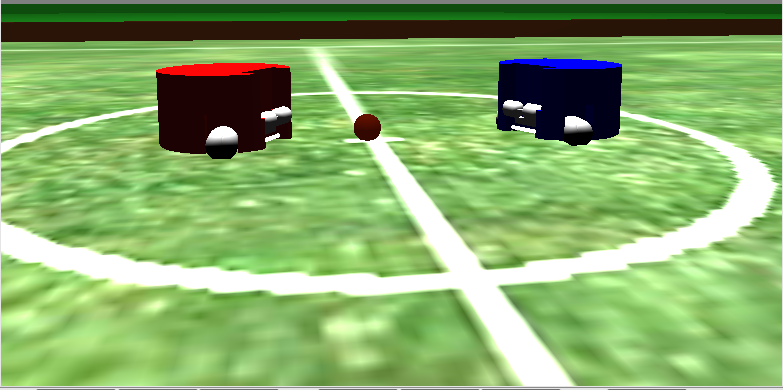
\includegraphics[scale=0.4]{./gazebo/roboty}
	\caption{Opracowane modele robotów  \label{fig:robots}}
	\end{figure}
	Robot został dodatkowo wyposażony w \textit{dribbler}\protect\footnote{urządzenie opisano w par.~\ref{sec:budowa_robota}} pomagający utrzymać kontrolę nad piłką.
	Mimo że \textit{Gazebo} udostępnia sterownik dla napędu holonomicznego, sterowanie robotem wymagało napisania nowego kontrolera, ponieważ nie uwzględniał on obsługi
	\textit{dribblera}, ani nie umożliwiał oddawania strzałów. Sterownik został zrealizowany w oparciu o teorię zawartą w rozdziale \ref{chap:holonomic}. Użytkownik  Dodatkowo zaimplementowano
	programowy regulator \texttt{PID}, sterujący siłą przykładana do kół robota. Dzięki temu uzyskano lepszą dokładość sterowania robotem. Parametry regulatora początkowo dobrano posługując się metodą \texttt{Zieglera-Nicholsa}, a następnie eksperymentalnie dokonano ich korekty.
	W pliku opisującym model robota istnieje możliość ich ręcznego modyfikowania.
	Kod źródłowy sterownika został zamieszczony na płycie CD razem z kodem źródłowym wykorzystywanej wersji symulatora.	
	\begin{figure}[H]
	\centering
	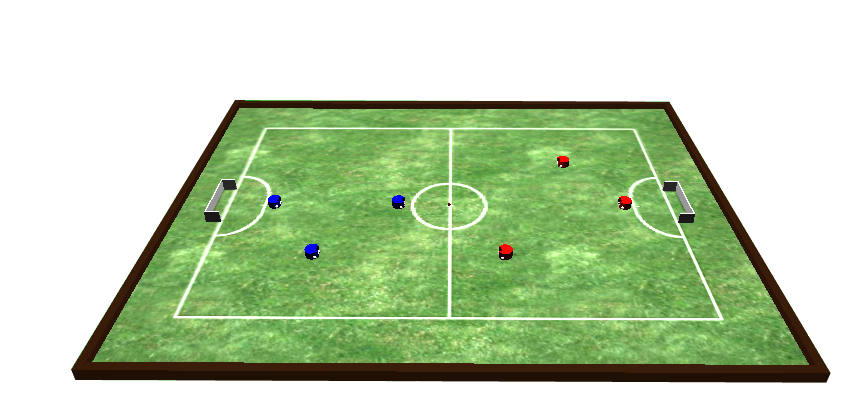
\includegraphics[scale=0.4]{./gazebo/boisko.png}
	\caption{Model boiska}
	\end{figure}
	W trakcie symulacji opracowanych modeli zauważono, że piłka raz wprawiona w ruch nie hamuje. Sytuacja taka była spowodowana brakiem tarcia tocznego. Zaimplementowano zatem kolejną modyfikację w 
	symulatorze, tak aby dla każdej bryły istniała możliwaść konfigurowania tego parametru (\textit{angularDamping}) w pliku opisującym model.

	Ponieważ korzystano z niestabilnej wersji oprogramowania (inne nie było jeszcze dostępne), pobranego bezpośrednio z repozytorium deweloperów, należało poprawić jeszcze kilka innych błędów symulatora,
	miedzy innymi niepoprawną pracę interfesju umożliwiającego komunikację pomiędzy symulatrem a aplikacją kliencką.

\chapter[Sterowanie modelem robota z \emph{Small-size League}]{Sterowanie modelem robota z \emph{Small-size League} \label{chap:holonomic}}
%\chaptermark{holonomic}
Budowę i napęd robota należy dobrać odpowiednio do postawionego zadania. W przypadku ligi \emph{Small-size League}, najważniejszym elementem jest prostota i mobilność
takiej jednostki, w pracy inżynierskiej \cite{inzynierka} posługiwano się robotem modelem robota o napędzie różnicowym (dwa niezależnie napędzane koła). Decyzję o odwzorowaniu takiego robota
w symulatorze motywowano wtedy próbą odzwierciedlenia rzeczywistego robota \texttt{HMT} \cite{hamada_mgr} stworzonego w ramach koła robotyki \texttt{Bionik} działającego na Wydziale Elektroniki i Technik Informacyjnych Politechniki
Warszawskiej. W niniejszej pracy zrezygnowano jednak z tego modelu, ponieważ nie był wystarczająco funkcjonalny. Zdecydowano się natomiast na zbudowanie modelu wzorowanego na rzeczywistym zawodniku \emph{Small-size League}.  
\section{Omówienie omnikierunkowej bazy jezdnej}
Analogicznie jak podczas rzeczywistej rozgrywki, decydującym elementem jest budowa anatomiczna i zdolności motoryczne zawodników, tak samo podczas
rozgrywek robotów istotna rolę odgrywa baza jezdna zawodników. W pracy inżynierskiej testom poddawany był robot o napędzie różnicowym. Baza ta posiadała jednak 
znaczące ograniczenia, które musiały zostać uwzględnione w algorytmach sterujących. Praktyczniejszą w użyciu jest baza omnikierunkowa. Korzystając z takiej bazy w
wiekszości algorytmów robot może być traktowany jako punkt materialny.
\subsection{Opis położenia kół}
Baza omnikierunkowa składa się z umieszczonych symetrycznie co najmniej trzech kół szwedzkich tak jak zaprezentowano to na rysunku \ref{fig:holonomic_base}.
Każde z kół posiada osobny napęd. Budowę koła omnikierunkowego przedstawiono na ilustracji \ref{fig:omnidirectional_wheel}. 
\begin{figure}[h]
\centering
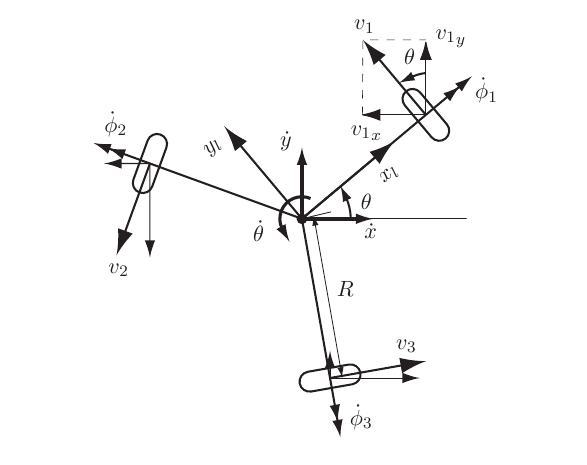
\includegraphics[scale=0.7]{./holonomic/holonomic_base}
\caption{ Rozkład kół w omnikierunkowej bazie jezdnej }\label{fig:holonomic_base}
\end{figure}
Koło szwedzkie posiada na swoim
obwodzie zamontowane w odpowiedni sposób dodatkowe rolki. Umożliwiają one ruch koła w dowolnym kierunku, bez względu na to, 
jak koło jest zorientowane w przestrzeni. Dzięki temu umożliwia ruch robota w dowolnym kierunku, czyli należy do klasy robotów holonomicznych.
\begin{figure}[h]
\centering
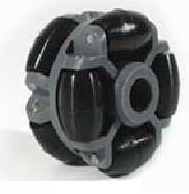
\includegraphics[scale=0.7]{./holonomic/omnidirectional_wheel}
\caption{ Konstrukcja przykładowego koła szwedzkiego }\label{fig:omnidirectional_wheel}
\end{figure}
\subsection{Opis kinematyki oraz dynamiki bazy}
Podczas sterowania robotem istotnym problemem jest sposób w jaki prędkości i przyspieszenia obrotowe poszczególnych kół przekładają się
na predkość/przyspieszenie kątowe i liniowe całego robota. Wszytskie poniższe obliczenia zostały wykonane przy założeniu, że koła nie ulegają poślizgowi,
czyli że cały moment obrotowy śilników przekłada się na prędkość robota.
Przyspieszenie liniowe i prędkość obrotowa środka masy takiego układu dane jest następującymi wzorami:
\begin{equation}
a=\frac{1}{M}(F1+F2+F3)
\end{equation}

\begin{equation}
\dot{ \omega }=\frac{R}{I}(f_1+f_2+f_3)
\end{equation}
, gdzie $f_i$ oznacza długość wektora siły przyłożonego do poszczególnego koła, a $I$  jest momentem bezwładności.
Przyspieszenie wzdłuż poszczególnych osi można obliczyć rozbijając siłę działającą na koło wzdłuż tychże osi, otrzymamy wtedy:
\begin{equation}
Ma_x=-f_1sin\theta_1 - f_2sin\theta_2 - f_3sin\theta_3
\end{equation}
\begin{equation}
Ma_y=f_1cos\theta_1 + f_2cos\theta_2 + f_3cos\theta_3
\end{equation}
Dla jednolitego cylindra moment bezwładności obliczany jest ze wzoru $I=\frac{1}{2}MR^2$, natomiast dla obręczy $I=MR^2$, gdzie $R$ jest odpowiednio promieniem
\mbox{cylindra/obręczy} natomiast $M$ masą. Dla obiektów o rozkładzie masy pomiędzy
obręczą, a cylindrem wprowadzany jest dodatkowy parametr $\alpha$. Wzór przyjmuje wtedy postać: $I=\alpha MR^2$, gdzie $0<\alpha<1$.
Używając zapisu macierzowego równania można przedstawić w postaci:
\begin{equation}
 \begin{pmatrix}
  a_x\\
  a_y\\
  \dot{\omega}
 \end{pmatrix}
  =
\begin{pmatrix}
  -sin\theta_1 & -sin\theta_2 & -sin\theta_3 \\
  cos\theta_1 & cos\theta_2 & cos\theta_3 \\
  \frac{MR}{I} & \frac{MR}{I} & \frac{MR}{I}\\
 \end{pmatrix} 
 \begin{pmatrix}
  f_1\\
  f_2\\
  f_3
 \end{pmatrix}
\end{equation}

Podstawiając do powyższego wzoru $I=\alpha MR^2$ oraz zastępując $\dot{\omega}$ wyrażeniem $R\dot{\omega}$ otrzymujemy:
\begin{equation}
 \begin{pmatrix}
  a_x\\
  a_y\\
  R\dot{\omega}
 \end{pmatrix}
  =
\begin{pmatrix}
  -sin\theta_1 & -sin\theta_2 & -sin\theta_3 \\
  cos\theta_1 & cos\theta_2 & cos\theta_3 \\
  \frac{1}{\alpha} & \frac{1}{\alpha} & \frac{1}{\alpha}\\
 \end{pmatrix} 
 \begin{pmatrix}
  f_1\\
  f_2\\
  f_3
 \end{pmatrix}
\end{equation}

Macierz z powyższego równania o wymiarze $3x3$ zostanie oznaczona symbolem $C_{\alpha}$.

Jednak najbardziej interesujący jest sposób w jaki prędkość obrotowa kół przekłada się na prędkość liniową robota.
Załóżmy, że robot porusza się wzdłuż osi OX, zatem wektor prędkości $(\upsilon_{x}, \upsilon_{y}, R\omega)$ wygląda następująco $(1,0,0)$.
Rozważmy jedno z kół, tak jak to przedstawiono na rysunku \ref{fig:linear_speed}, dokonując rozkładu wektora prędkości na dwie składowe, jedną zgodną z ruchem
obrotowym dużego koła, a drugą zgodną z ruchem małych, poprzecznych kółek otrzymujemy odpowiednio prędkości $\upsilon=-sin\theta$ $\upsilon_{y}=cos\theta$.
Przy wyznaczaniu prędkośći koła przyjęto założenie, że prędkość dodatnia powoduje obrót w kierunku wyznaczonym przez kciuk prawej dłoni, gdy pokrywa się ona z osią 
silnika.
Otrzymujemy zatem następujące powiązanie pomiędzy prędkościami robota, a prędkościami poszczególnych silników:
 \begin{equation}
 \begin{pmatrix}
  \upsilon_1\\
  \upsilon_2\\
  \upsilon_3
 \end{pmatrix}
  =
\begin{pmatrix}
  -sin\theta_1 & cos\theta_1 & 1 \\
  -sin\theta_2 & cos\theta_2 & 1 \\
  -sin\theta_3 & cos\theta_3 & 1 \\
 \end{pmatrix} 
 \begin{pmatrix}
  \upsilon_x\\
  \upsilon_y\\
  R\omega
 \end{pmatrix}
\end{equation}
\begin{figure}[h]
\centering
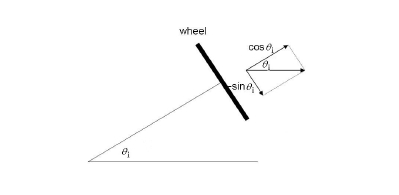
\includegraphics[scale=0.7]{./holonomic/linear_speed}
\caption{ Prędkość liniowa dużego koła szwedzkiego i małych kółek, gdy robot porusza się wzdłuż osi OX }\label{fig:linear_speed}
\end{figure}

\section{Obliczanie profilu prędkości liniowej robota}
Znając już powiązanie pomiędzy prędkością obrotową kół a prędkością liniową i obrotową robota, ostatnim elementem jest wyznaczenie prędkości prowadzących 
robota do zadanego punktu. Należy przy tym uwzględnić takie parametry robota jak przyspieszenie i opóźnienie. W tym celu skorzystano z metody opisanej w 
\cite{trapezy1} oraz \cite{trapezy2}. Polega ona na dekompozycji dwuwymiarowego problemu sterowania robotem, do dwóch problemów jednowymiarowych, tak jak to zaprezentowano
na rysunku \ref{fig:trapezoid_rule}. Ruch robota w kierunku osi OX i w kierunku osi OY jest rozpatrywany osobno. 
\begin{figure}[H]
\centering
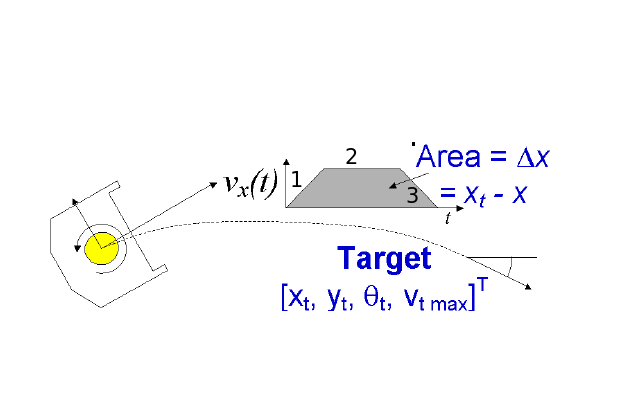
\includegraphics[scale=0.7]{./holonomic/trapezoid_rule}
\caption{ Dekompozycja sterowania robotem w 2D na dwa niezależne zadania w 1D }\label{fig:trapezoid_rule}
\end{figure}
Podejście to jest znane w robotyce pod nazwą trapezoidalnego profilu prędkości.
Zaczynając od punktu w którym robot się znajduje przyspiesza on
ze swoim stałym przyspieszeniem, aż do osiągnięcia maksymalnej prędkości, następnie zaczyna hamować, tak aby zatrzymać się w punkcie docelowym.
W szczególnym przypadku profil prędkości może przybrać formę trójkąta.
Prędkość obliczana jest według następujących reguł:
\begin{enumerate}
\item Jeśli bieżąca prędkość spowoduje oddalenie się robota od celu to wyhamuj do 0.
\item Jeśli robot poruszając się z bieżąca prędkością przejedzie cel to także należy zatrzymać go.
\item Gdy bieżąca prędkość przekracza maksymalną, wyhamuj do prędkości maksymalnej.
\item Oblicz trójkątny profil prędkości prowadzącej do celu.
\item Jeśli w obliczonym rozkładzie prędkość przekracza w jakimkolwiek momencie maksimum to należy obliczyć trapezoidalny profil. 
\end{enumerate} 

\section{Dryblowanie z piłką}
\todo{opiać matematykę dryblowania z piłką}
\begin{itemize}
 \item ograniczenia wynikające z budowy \texttt{dribblera},
 \item wyznaczanie dopuszczalnych prędkośći.
\end{itemize}



\chapter{Algorytmy unikania kolizji \label{chap:algorytmy}}
 W rozdziale zostanie szerzej zaprezentowany jeden z algorytmów unikania kolizji jakim jest RRT(\texttt{Rapidly-Exploring Random Tree}).
Poruszona zostanie także kwestia powodów, dla których wybrano tę, a nie inną metodę. Uzasadnione zostanie odejście od algorytmu opracowanego w ramach pracy 
inżynierskiej (CVM \texttt{Curvature Velocity Method}). Ponadto opisane zostaną inne metody planowania ścieżki oraz omówione zostaną ich właściwości. Na tej podsatwie zostanie 
uzasadniony wybór algorytmu RRT.

\section{Krótki przegląd algorytmów unikania kolizji}
Jednym z podstawowych problemów podczas poruszania się każdej jednostki mobilnej jest wyznaczenie bezkolizijnej ścieżki prowadzącej do celu.
Współczesna robotyka zna wiele algorytmów rozwiązujących z mniejszym bądź większym sukcesem to zadanie. Użycie wielu z nich jest jednak w pełni uzasadnione tylko w
szczególnych okolicznościach.Poniżej zostaną zaprezentowane najbardziej znane algorytmy unikania kolizji (omówione także w pracy inżynierskiej \cite{inzynierka}
\subsection{Algorytm Bug}
	Najprostszym algorytmem unikania kolizji jest algorytm \emph{Bug}, naśladujący zachowanie pluskwy. Gdy robot,
	podążając do punktu docelowego napotyka przeszkodę, okrąża ją całkowicie i zapamiętuje położenie w którym
	znajdował się najbliżej celu. Następnie ponownie podczas powtórnego okrążania przeszkody robot dąży do
	uprzednio zapamiętanego punktu po czym odrywa się od przeszkody i zaczyna podążać w stronę celu. Ścieżka
	wyznaczona za pomocą algorytmu została zaprezentowana na rysunku
	\ref{fig:Bug1}. Robot wykorzystujący ten algorytm powinien być wyposażony w dwa rodzaje czujników:
	\begin{itemize}
	\item czujnik celu -- wskazujący kierunek do celu oraz umożliwiający pomiar odległości do celu
	\item czujnik lokalnej widoczności -- umożliwiający  podążanie wzdłuż konturu przeszkody 
	\end{itemize}
	\begin{figure}[h]
	\centering
	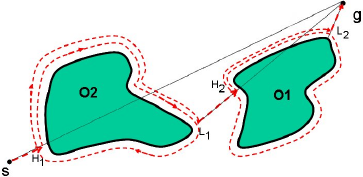
\includegraphics[scale=0.7]{./algorytmy/Bug1}
	\caption{ Bezkolizyjna ścieżka wyznaczona przez algorytm Bug }\label{fig:Bug1}
	\end{figure}
	Ścieżka wyznaczona przez ten algorytm jest daleka od optymalnej. Robot niezależnie od wybranego kierunku
	omijania przeszkody musi ją okrążyć całkowicie. W pewnych sytuacjach całkowite okrążenie przeszkody jest niemożliwe, np jesli przeszkodą jest ściana. W takim przypadku algorytm zawodzi całkowicie.
	Efektywność algorytmu można poprawić sprawdzając podczas okrążania przeszkody czy punkt w którym aktualnie
	znajduje  się robot jest poszukiwanym punktem położonym najbliżej celu. Przykładowa ścieżka
	wyznaczona za pomocą zmodyfikowanej wersji algorytmu jest widoczna na rysunku \ref{fig:Bug2}.
	Robot otacza przeszkodę w wybranym wcześniej kierunku i odłącza się od niej w momencie przecięcia
 	prostej łączącej punkt startowy z punktem docelowym. Uzyskana w ten sposób ścieżka nadal zależy od wybranego
	 a priori kierunku jazdy.	
	\begin{figure}
	\centering
	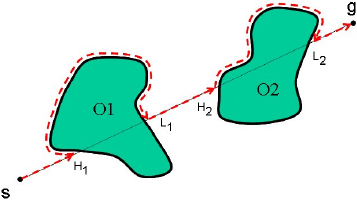
\includegraphics[scale=0.7]{./algorytmy/Bug2}
	\caption{Zasada działania algorytmu Bug w wersji rozszerzonej}\label{fig:Bug2}
	\end{figure}
	Obie zaprezentowane wersje algorytmu Bug nie uwzględniaja ograniczeń wynikających z kinematyki robota, a w
	szczególności faktu, że rozpatrywany robot może być nieholonomiczny.
\subsection{Algorytm VHF}
	Pełna  anglojęzyczna nazwa metody brzmi \mbox{ \emph{Vector Field Histogram}}, na język polski można ją
	przetłumaczyć jako algorytm histogramu pola wektorowego. Należy ona do grupy metod, które w czasie
	rzeczywistym pozwalają na jednoczesne wykrywanie i omijanie przeszkód oraz kierowanie robota na cel.
	Algorytm ten został szczegółowo opisany w pracy inżynierskiej \cite{inzynierka}, więcej informacji można też znaleźć w publikacjach autorów, \cite{VFH_1} oraz \cite{VFH_2}.
	W skrócie jego zasada działania opiera się na konstrukcji dwuwymiarowego opisu świata w postaci siatki. Każdemu elementowi siatki przypisany jest poziom ufności oddający prawdopodobieństwo
	z jakim w danym położeniu może pojawić się przeszkoda (rysunek \ref{fig:VFH_siatka}).
	\begin{figure}[H]
	\centering
	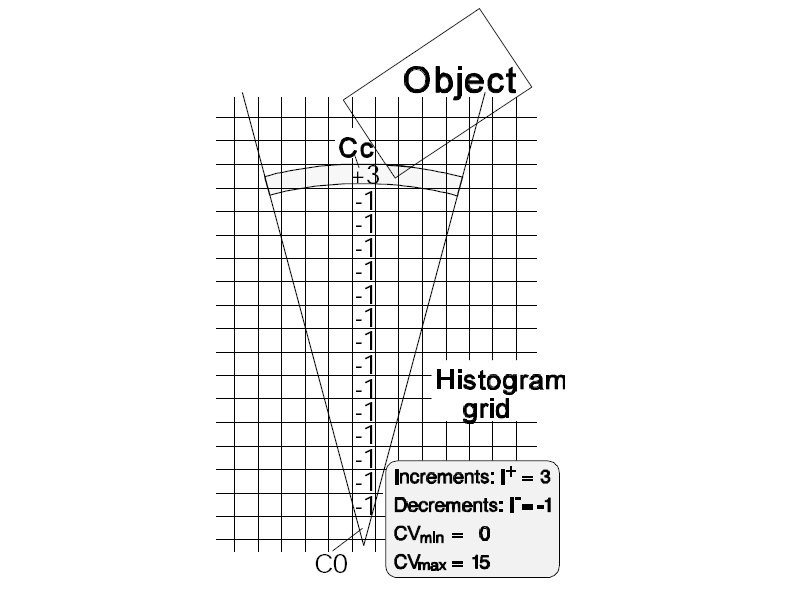
\includegraphics[scale=0.44]{./algorytmy/VFH_siatka}
	\caption{ Zasada tworzenia dwuwymiarowego histogramu \newline(na podstawie \cite{VFH_2})}\label{fig:VFH_siatka}
	\end{figure}
	Tak skonstruowana mapa redukowana jest do jednowymiarowego histogramu biegunowego (rysunek \ref{fig:VFH_hist_biegunowy}), który dodatkowo wygładzany jest przez
	filtr dolnoprzepustowy. W ten sposób otrzymuje się informację o poziomie ufności wystąpienia przeszkody poruszając się w danym kierunku (świadomomie rezygnuje się z informacji o odległości od przeszkody).
	Na podstawie tego histogramu wyznaczane są sterowania dla robota. Histogram jest analizowany w poszukowaniu minimów lokalnych, wszystkie doliny, których poziom ufności
	znajduję się poniżej ustalonego umownie progu są rozważane przy wyznaczaniu kierunku jazdy robota. Jeśli minimów jest kilka wybierane jest to, którego kierunek prowadzi najbliżej
	do celu. 
	Do poprawnego działania algorytm potrzebuje informacji o rozłożeniu przeszkód w otoczeniu robota, w oryginalnej implementacji była ona pozyskiwana z sensorów ultradźwiękowych,
	można je zastąpić z powodzeniem czujnikami laserowymi. Obraz video z kamery umieszczonej nad eksplorowanym światem także dostarcza tej informacji (jak w rozgrywkach \emph{Small-size League}).
	\begin{figure}[H]
	\centering
	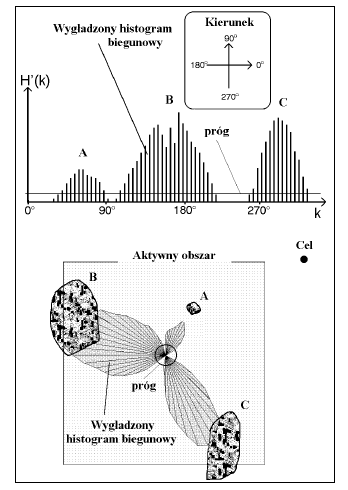
\includegraphics[scale=0.5]{./algorytmy/VFH_hist_biegunowy}
	\caption{ Histogram biegunowy dla przykładowego rozmieszczenia przeszkód \newline(na podstawie \cite{ISR})}\label{fig:VFH_hist_biegunowy}
	\end{figure}

	\subsection{Technika dynamicznego okna} \label{subsec:dynamic_window}
	Popularną, stosowaną w robotyce metodą unikania kolizji jest także technika dynamicznego okna. Algorytm ten analizuje jedynie możliwe do osiągnięcia w danej sytuacji prędkości.
	Więcej informacji na temat algorytmu można znaleźć w publikacji \cite{dynamic_window} lub w pracy inżynierskiej \cite{inzynierka}.
	Ujmując w jedym zdaniu algorytm polega na przeszukiwaniu zbioru dopuszczalnych prędkości liniowych i kątowych, tak aby maksymalizować funkcję celu. Sposób konstrukcji funkcji celu
	gwarantuje, że wybrane prędkości będą prowadzić robota w zamierzonym kierunku oraz, że nie natrafi na przeszkodę.
\subsection{Algorytmy pól potencjałowych}
\subsubsection{Algorytm w wersji podstawowej}
	Kolejne podejście do problemu nawigacji robota mobilnego zaczerpnięto z fizyki. Problem znalezienia bezkolizyjnej ścieżki został sprowadzony do problemu konstrukcji
	funkcji opisującej rozkład energii w danym środowisku. W takim układzie dotarcie do celu jest równoważne ze znalezieniem minimum funkcji opisującej rozkład sztucznego pola
	potencjałowego. Robot podąża w kierunku ujemnego gradientu tej fukncji, mamy zatem $c(t)=- \nabla U(c(t))$. W klasycznym podejściu sztuczne pole potencjałowe tworzy
	się w ten sposób, że przeszkody są źródłem ujemnego pola(odpychającego), natomiast cel emituje pole dodatnie. Ujęte jest to w następujących wzorach:
	\begin{equation}
	U(q) = U_{att}(q) + U_{rep}(q)
	\end{equation}
	\begin{equation}\label{eq:CVM_dv}
		U_{att}(q) = \left\{ 
		\begin{array}{l l}
		\frac{1}{2}\xi d^2 & \quad \mbox{dla $d\leqq d^{*}_{goal}$ }\\
		\xi d^{*}_{goal}d - \frac{1}{2}(d^{*}_{goal})^{2} & \quad \mbox{dla $d\geqq d^{*}_{goal}$ }\\
		\end{array} \right. 
	\end{equation}
	, gdzie $d=d(q,q_{goal})$ jest odległością danego położenia od celu, $\varepsilon$ jest stałą określającą poziom przyciągania do celu, natomiast $d^{*}_{goal}$ określa próg,
	po którym funkcja z kwadratowej przechodzi w trójkątną.
	Oddziaływanie przeszkód opisane jest następującym wzorem:
	\begin{equation}
		U_{rep}(q) = \left\{ 
		\begin{array}{l l}
		\frac{1}{2} \eta{ ( \frac{1}{D(q)} - \frac{1}{ Q^{*} } )}^2  & \quad \mbox{dla $D(q)\leq Q^{*} $ }\\
		0 & \quad \mbox{dla $D(q)> Q^{*}$ }\\
		\end{array} \right.
	\end{equation}
	,gdzie $ Q^{*} $ jest zasięgiem pola odpychającego przeszkody, natomiast $\eta$ odpowiada za siłę tego pola. 
	Kierunek w którym podążać ma robot wyznaczany jest ze wzoru:
	\begin{equation}
	- \nabla U(q) = - \nabla U_{att}(q) - \nabla U_{rep}(q)
	\end{equation}
	Powyższe podejście w stosunkowo prosty sposób umożliwa wyznaczenie kierunku bezkolizyjnej ścieżki do celu, jednak posiada pewną dość istotną wadę, mianowicie w pewnych, 
	szczególnych sytuacjach robot może utknąć w minimum lokalnym. Sposób w jaki konstruowana jest funkcja celu w żaden sposób nie wyklucza występowania minimów lokalnych.
	W przypadku, gdy sterowany robot utknie w lokalnym minimum, konieczna jest reakacja ze strony wyższej warstwy nawigującej maszyną, przykładowo można wykorzystać algorytm 
	błądzenia losowego.
\subsubsection{Funkcja nawigacji}
	Istnieje jednak pewna szczególna funkcja, która posiada tylko globalne minimum, została ona zdefiniowana w publikacjach \cite{navi_func1},\cite{navi_func2}.
	Przykładowy wykres funkcji nawigacji jest zamieszczony poniżej (rysunek ~\ref{fig:func_navi}). Zasięg oddziaływania minimum globalnego zależy od kilku istotnych parametrów, które zawarte są 
	we wzorze opisującym rozkład sztucznego potencjału.
		\begin{figure}[!h]
		\centering
		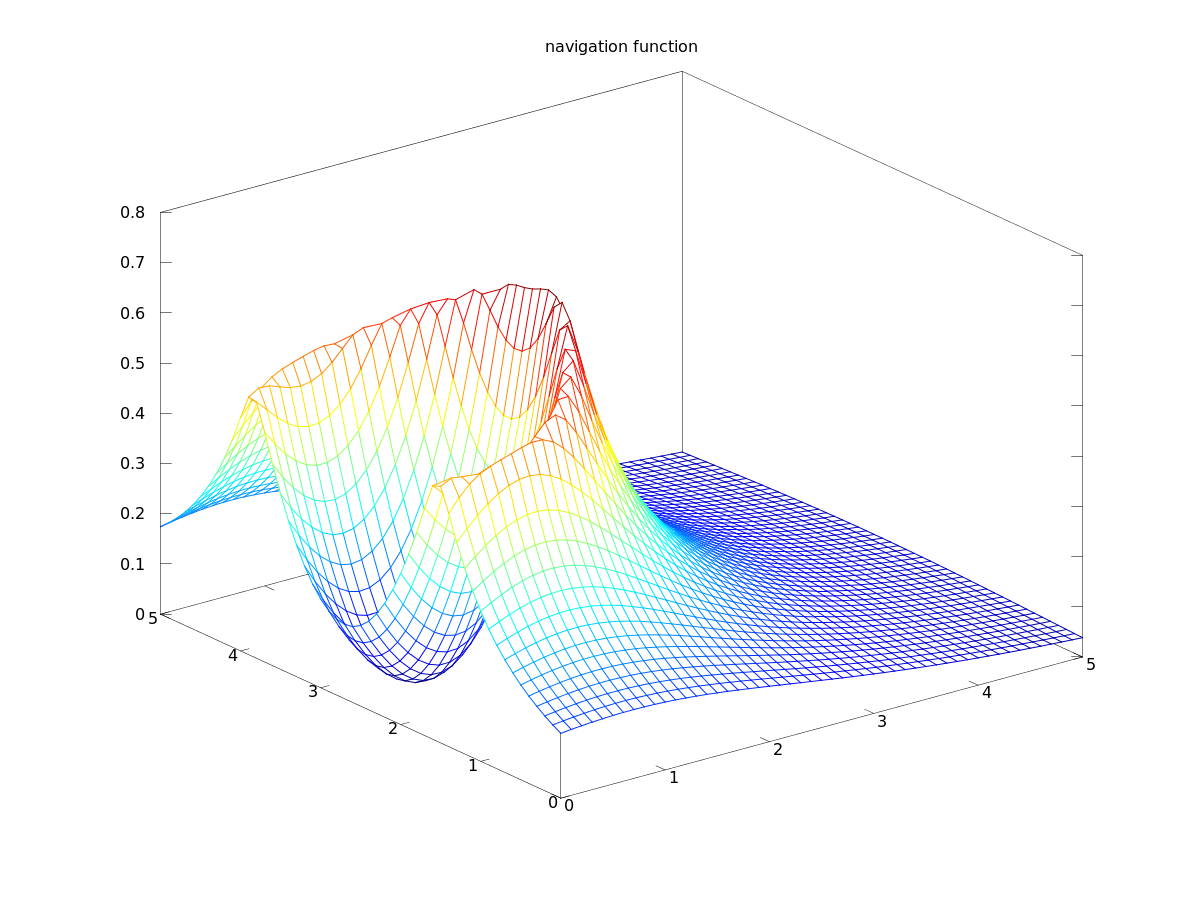
\includegraphics[scale=0.3]{./algorytmy/navigation_func_k_10}
		\caption{Funkcja nawigacji dla $\kappa=10$}
		\label{fig:func_navi}
		\end{figure}
	Dla bieżącego położenia robota $q$ funkcja nawigacji zdefiniowana jest następująco:
	\begin{equation}
	\label{eq:navi_func}
	\phi = \frac{(d(q,q_{goal}))^2}{ (\lambda \beta(q) + d(q,q_{goal})^{2\kappa} )^{\frac{1}{\kappa}}}
	\end{equation}
	gdzie $\beta(q)$ jest iloczynem funkcji odpychających zdefiniowanych dla wszytskich przeszkód:
	\begin{equation}
	\beta  \stackrel{ \vartriangle }{ = } \prod_{i=0}^{N}{ \beta_i(q)}    
	\end{equation}
	Natomiast dla każdej przeszkody($i>0$) funkcja określona jest następująco:
	\begin{equation}
	\beta_{i}(q)=(d(q,q_i))^2 - r_i^{2} \text{ dla i = 1...N, gdzie N jest liczbą przeszkód}
	\end{equation}
	Powyższa funkcję definiuje się dla każdej z przeszkód o promieniu $r_i$, której środek znajduje się w punkcie $q_i$.
	Jak łatwo zauważyć, funkcja ta przyjmuje ujemne wartości wewnątrz okręgu opisującego przeszkodę, natomiast dodatnie na zewnątrz okęgu.
	Dodatkowo definiuje się funkcję $\beta_{0}(q)= -(d(q,q_0))^{2} + r_0^{2}$, w której parametry $r_0$ oraz $q_0$ oznaczają odpowiednio promień świata w którym porusza się robot
	oraz środek tego świata.
	Wzór \ref{eq:navi_func} posiada dwa istotne parametry, $\lambda$ ogranicza przeciwdziedzinę do przedziału $[0,1]$, gdzie wartość $0$ jest tożsama z osiągnięciem celu, natomiast
	$1$ jest osiągna na brzegu każdej z przeszkód. Drugi parametr $\kappa$ odpowiednio dobrany powoduje, że blisko celu wykres funkcji $\phi$ przybiera kształt misy.
	Zwiększanie parametru $\kappa$ powoduje przesuwanie globalnego minimum w kierunku położenia punktu docelowego, zwiększa zatem oddziaływanie przyciągającego pola emitowanego przez 
	punkt docelowy.

	Wykres funkcji nawigacji przedstawiony na rysunku \ref{fig:func_navi} został sporządzony dla następujących parametrów(wszystkie jednostki wyrażone są w metrach):
	\begin{enumerate}
	\item eksplorowany świat ograniczony jest okręgiem o środku w punkcie $q_0(2.7;3.7)$ i promieniu $r_0 = 7.4$,
	\item $\lambda = 0.2$,
	\item $\kappa = 10$,
	\item przeszkody umiejscowione są w punktach $(2;2),(3;3)(4;4),(3.5;3.5)$ i mają stały promień, odpowiadający modelowi robota
	zastosowanemu podczas doświadczeń $r_i = 0.14 $,
	\item punkt docelowy ma współrzędne $q_g(2.7;0.675)$,
	\item funkcja nawigacji została wykreślona z krokiem $0.1$.
	\end{enumerate}

\subsection{Algorytm CVM (\texttt{Curvature Velocity Method})}
	W pracy inżynierskiej \cite{inzynierka} jako docelowy algorytm unikania kolizji wybrany został właśnie \texttt{CVM}.
	Metoda krzywizn i prędkości (ang. \textit{Curvature Velocity Method}) została zaproponowana przez R. Simmonsa w
	\cite{CVM_2}, należy do grupy metod bazujących na przeszukiwaniu przestrzeni prędkości, a jej działanie
	jest zbliżone do techniki dynamicznego okna zaprezentowanej w \ref{subsec:dynamic_window}.

	Spośród wszystkich par $(v,\omega)$ wybierana jest taka, która osiąga największą wartość funkcji celu.
	Podejście takie umożliwia uwzględnienie przede wszystkim ograniczeń kinematycznych, ale także i dynamicznych.
	Wyznaczone przez algorytm sterowanie na następny krok definiuje łuk $c=\frac{\omega}{v}$, po którym będzie
	poruszał się robot do chwili wyznaczenia kolejnego sterowania.
	
	Funkcja celu została tak skonstruowana, aby preferować prędkości, które prowadzą do celu, ale jednocześnie  
	nie powodują kolizji. Ponadto dołożone zostało kryterium na maksymalizację prędkości liniowej robota. Funkcja celu jest zatem sumą ważoną trzech składowych: 
	\begin{equation} \label{eq:fcelu_cvm}
	F(v,\omega)=\alpha_1 \mathcal{V}(v,\omega)+\alpha_2 \mathcal{D}(v,\omega) + \alpha_3 \mathcal{G} (v,\omega))
	\end{equation}
	gdzie:
	\begin{itemize}
	 \item $\alpha_1, \alpha_2, \alpha_3$ współczynniki wagowe,
	 \item funkcja $\mathcal{V}(v,\omega)$ określa stosunek między ocenianą prędkością liniową a maksymalną,
	 \item funkcja $\mathcal{D}(v,\omega)$ określa odległość od najbliższej przeszkody na którą napotka robot poruszający się po trajektorii wyznaczonej przez $(v,\omega)$,
	 \item funkcja $\mathcal{G}(v,\omega)$ odpowiada za kierowanie się robota na cel.
	\end{itemize}
	Zachowaniem robota można sterować poprzez zmianę wartości współczynników wagowych. W skrajnych przypadkach,
	gdy któryś ze współczynników zostanie wyzerowany, traci on całkowicie wpływ na trajektorię po której
	porusza się robot. Szczegółowy opis poszczególnych składowych, jak i samego działania metody został
	zaprezentowany w paragrafie \ref{sec:CVM:action}.

	\section{Zasada działania CVM \label{sec:CVM:action}} 
	Omawianie mechanizmu wyboru najlepszego sterowania z wykorzystaniem algorytmu \textit{CVM} należy rozpocząć od przypomnienia funkcji celu (\ref{eq:fcelu_cvm})
	\begin{equation*}
	F(v,\omega)=\alpha_1 \mathcal{V}(v,\omega)+\alpha_2 \mathcal{D}(v,\omega) + \alpha_3 \mathcal{G} (v,\omega))
	\end{equation*}
	W powyższym równaniu składowe odpowiadające za kierowanie na cel oraz za maksymalizację prędkości liniowej zostały zdefiniowane następująco:
	\begin{gather}
	\mathcal{V}(v,\omega)=\frac{v}{V_{max}} \label{eq:CVM_speed}\\
	\mathcal{G}(v,\omega)=1-\frac{|\theta_{cel} -T_{alg}\omega|}{\pi} \label{eq:CVM_head}
	\end{gather}
	gdzie:
	\begin{itemize}
	 \item $V_{max}$ -- maksymalna prędkość liniowa z jaką może poruszać się robot
	 \item $T_{alg}$ -- czas na jaki wystawiane jest obliczone sterowanie
	 \item $\theta_{cel}$ -- orientacja do celu w układzie współrzędnych robota 
	\end{itemize}
	Natomiast zdefiniowanie składowej odpowiedzialnej za omijanie przeszkód wymaga określenia pewnych dodatkowych 
	funkcji wykorzystywanych w algorytmie. Należy dokonać przekształcenia opisu przeszkód we współrzędnych
	kartezjańskich  do przestrzeni prędkości. Dokonywane jest to za pomocą odległości do punktu $p$, w którym wystąpi kolizja z przeszkodą  $o$, jeśli robot będzie poruszał się po trajektorii $c=\frac{\omega}{v}$. Wartość ta jest oznaczana jako
	$d_c((0,0),p)$, gdzie $p$ jest punktem zderzenia z przeszkodą.
	Następnie należy zdefiniować funkcję odległości robota od przeszkody:
 	\begin{equation}\label{eq:CVM_dv}
	d_v(v,\omega,p)= \left\{ 
	\begin{array}{l l}
  	d_c((0,0),p_i & \quad \mbox{dla $v\neq0$}\\
  	\infty & \quad \mbox{dla $v=0$ }\\
	\end{array} \right. 
	\end{equation}
	Dla danego zbioru przeszkód $O$ zawsze wybierana jest odległość do najbliższej przeszkody leżącej na trajektorii. Zatem funkcję dla danego zbioru przeszkód $O$ można zapisać następująco:
 	\begin{equation}\label{eq:CVM_Dv}
	D_v(v,\omega,O)= \underset{o \in O}{\operatorname{inf}} d_v(v,\omega,o)
	\end{equation}
	W rzeczywistości jednak informacja o położeniu przeszkód jest ograniczona do pewnego obszaru, który może
	wynikać z zasięgu czujników w jakie wyposażony jest robot, bądź ze sztucznego ograniczenia zasięgu działania
	algorytmu w przypadku, gdy możliwy jest dostęp do globalnej informacji o położeniu przeszkód. Zasięg algorytmu  będzie  w dalszej część pracy oznaczany jako $L$. Funkcja  (\ref{eq:CVM_Dv})
	jest zatem ograniczona od góry w sposób następujący:
 	\begin{equation}\label{eq:CVM_Dv_ogr}
	D_{ogr}(v,\omega,P)= \min(L, D(v,\omega,P))
	\end{equation}
	Po uprzednim zdefiniowaniu niezbędnych funkcji  można podać postać funkcyjną składowej funkcji celu odpowiadającej za unikanie kolizji:
	\begin{equation} \label{eq:CVM_dist}
	\mathcal{D}(v,\omega)=\frac{D_{ogr}}{L}
	\end{equation}
 	
	Aby sposób obliczania odległości do przeszkody był możliwie jak najprostszy, każda przeszkoda jest
	reprezentowana w algorytmie jako okrąg o  promieniu \emph{r} (wynikającym z jej rozmiarów) i współrzędnych środka $(x_0,y_0)$. Można zatem dość łatwo wyznaczyć odległość, jaką przebędzie robot poruszający się po łuku wyznaczonym przez parę $(v,\omega)$ do
	momentu przecięcia z okręgiem. Zostało to zobrazowane na rysunku \ref{fig:CVM_dist}.
	\begin{figure}[!b]
	\centering
	%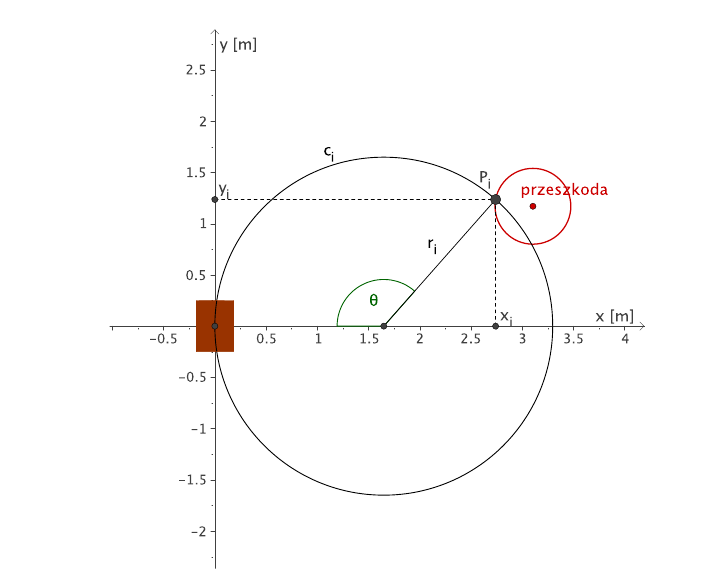
\includegraphics[scale=0.43]{./algorytmy/CVM_dist}
	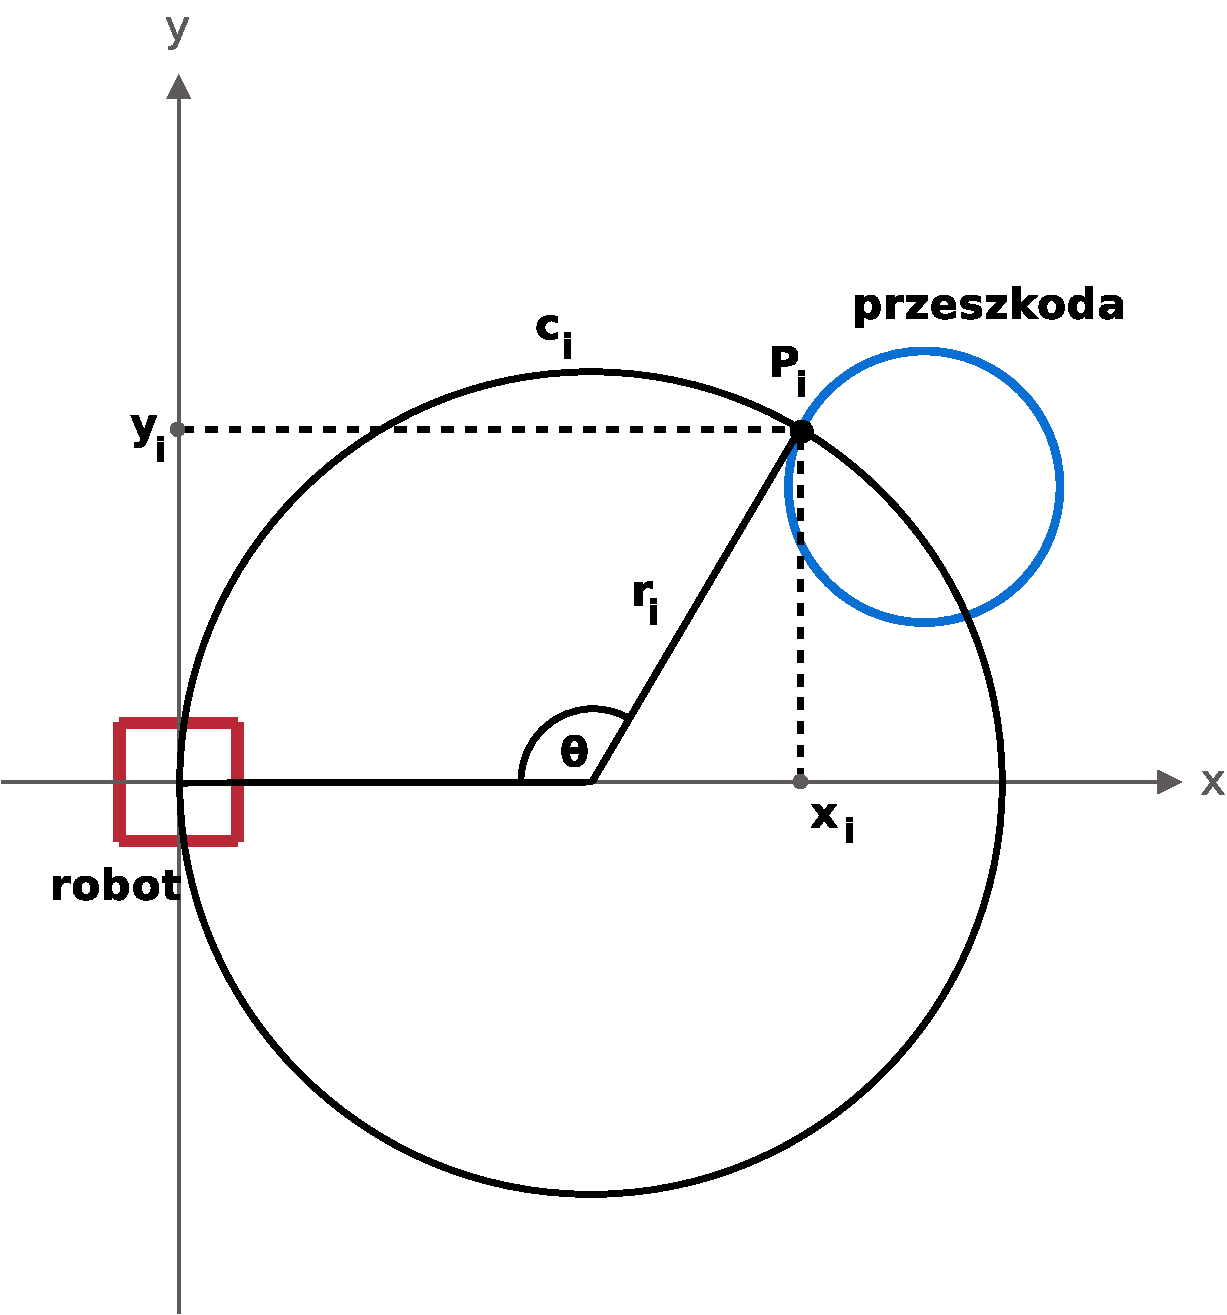
\includegraphics[scale=0.35]{./algorytmy/CVM_dist_new}
	\caption{ Obliczanie odległości od przeszkody \label{fig:CVM_dist}}
	\end{figure}
	
	Dla robota o początkowej orientacji zgodnej z osią $OY$, poruszającego się po trajektorii o krzywiźnie $c$ przecinającej
	okrąg opisujący przeszkodę w punkcie $P(x,y)$ prawdziwe są następujące wzory:
	\begin{equation}\label{eq:CVM_teta}
	\theta= \left\{ 
	\begin{array}{l l}
	\text{atan2}(y,x-\frac{1}{c} )& \quad \mbox{dla $c<0$}\\
  	\pi-\text{atan2}(y,x-\frac{1}{c}) & \quad \mbox{dla $c>0$}\\
	\end{array} \right. 
	\end{equation}
	
	\begin{equation}
	d_c((0,0),P)= \left\{ 
	\begin{array}{l l}
  	y& \quad \mbox{dla $c=0$}\\
  	|\frac{1}{c}|\theta & \quad \mbox{dla $c\neq0$}\\
	\end{array} \right. 
	\end{equation}
	Zastosowana we wzorze (\ref{eq:CVM_teta}) funkcja \emph{atan2} zwraca wartości z przedziału $[-\pi;\pi]$, zatem uwzględnia w której ćwiartce leży kąt:
	\begin{equation}\label{eq:atan2}
	\text{atan2}(y,x)= \left\{ 
	\begin{array}{l l}
	\arctan{\frac{|y|}{|x|}} \sgn{(y)} & \quad \mbox{dla $x>0$}\\
	\frac{\pi}{2}\sgn{(y)} & \quad \mbox{dla $x=0$}\\
	\pi-\arctan{\frac{|y|}{|x|}} \sgn{(y)} & \quad \mbox{dla $x<0$}\\
	\end{array} \right. 
	\end{equation}
	
	Jednakże obliczanie odległości od przeszkody dla każdego sterowania $(v,\omega)$ w sposób omówiony powyżej
	jest czasochłonne. Stąd konieczne jest kolejne uproszczenie. Łatwo zauważyć, że z punktu $(0,0)$ w którym
	znajduje się robot można poprowadzić dwa łuki styczne do okręgu opisującego przeszkodę $p$. Zatem na zewnątrz
	krzywych stycznych odległość  $d_c((0,0),p)$ jest nieskończona. Natomiast dla krzywizn zawierających się
	pomiędzy łukami stycznymi można dokonać przybliżenia wartością stałą. Omawiana sytuacja została zobrazowana na
	rysunku \ref{fig:CVM_styczne}.
	\begin{figure}[!b]
	\centering
	%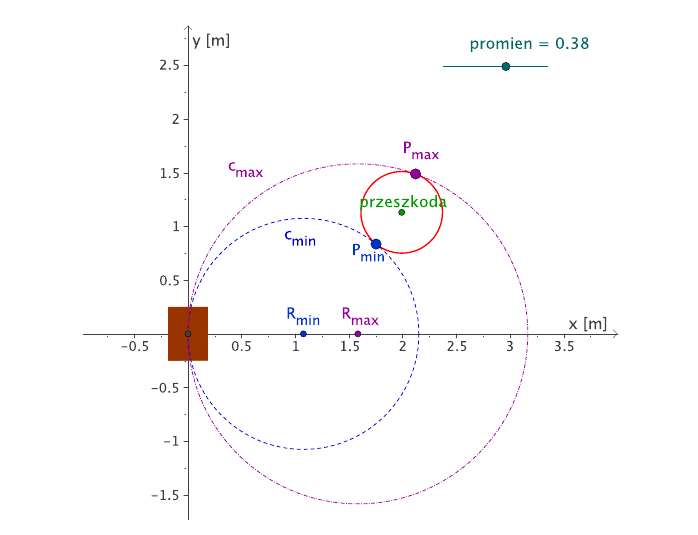
\includegraphics[scale=0.45]{./algorytmy/CVM_styczne}
	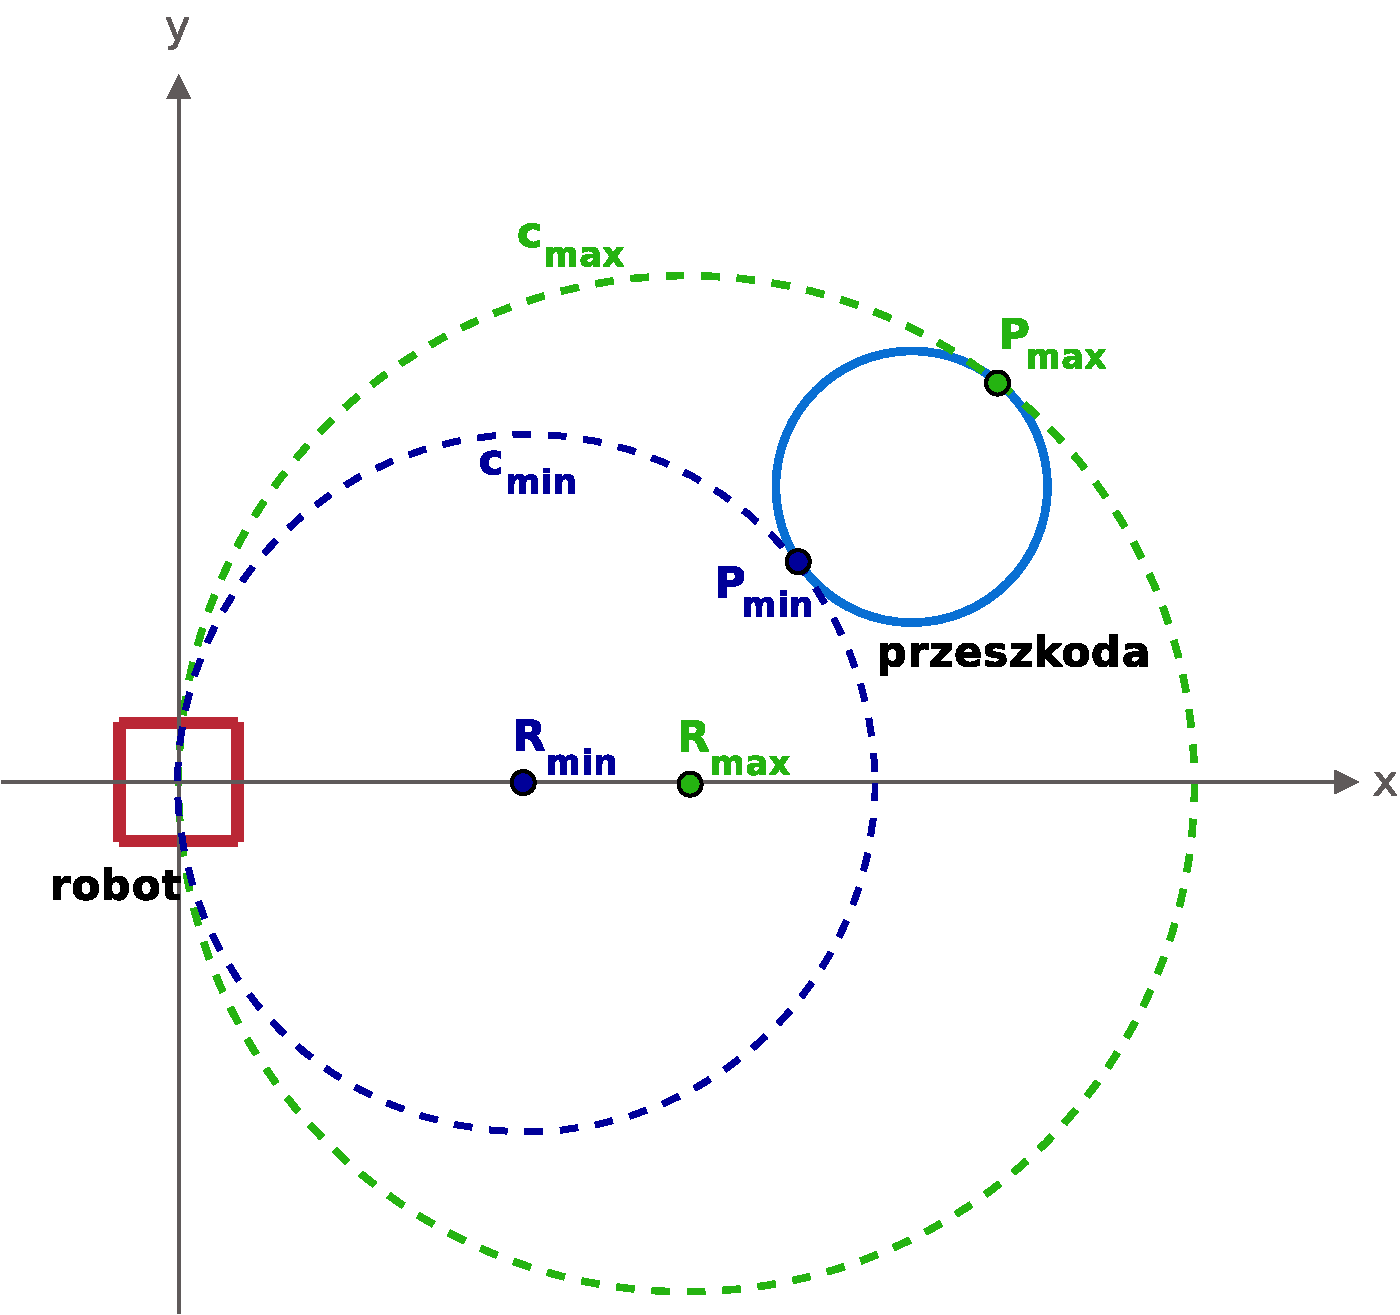
\includegraphics[scale=0.32]{./algorytmy/CVM_styczne_new}
	\caption{ Zasada wyznaczania przedziału $(c_{min}$,$c_{max})$ \label{fig:CVM_styczne}}
	\end{figure}
	Aby wyznaczyć okręgi styczne do okręgu opisującego przeszkodę należy znaleźć takie $r$ dla którego
	poniższy układ równań ma dokładnie jedno rozwiązanie:
	\begin{equation}\label{eq:CVM_styczne}
	 \left\{ 
	\begin{array}{l l}
  	(x-x_0)^2 + (y-y_0)^2={r_0}^2\\
  	 (x-r)^2 + y^2={r}^2\\
	\end{array} \right. 
	\end{equation}
	Gdzie $(x_0,y_0)$ jest środkiem okręgu opisującego przeszkodę, natomiast $r_0$ jego promieniem.
	W wyniku takiego postępowania można otrzymać punkty styczności $P_{max}$ oraz $P_{min}$ oraz odpowiadające im krzywizny $c_{min}$ oraz $c_{max}$. 
	Ostatecznie można już dokonać przybliżenia odległości po łuku od rozpatrywanej przeszkody $p$ w następujący sposób:
	\begin{equation}\label{eq:CVM_dv_const}
	d_v(v,\omega,p)= \left\{ 
	\begin{array}{l l}
  	\min(d_c((0,0),P_{max}),d_c((0,0),P_{min})) & \quad \mbox{$c_{min}\leq c \leq c_{max}$  }\\
  	\infty & \quad \mbox{w p.p. }\\
	\end{array} \right. 
	\end{equation}

	Zaprezentowane rozumowanie prowadzi do sytuacji, w której zbiorowi przeszkód $O$ odpowiada zbiór przedziałów krzywizn o stałej odległości od przeszkody. W dalszej części pracy przedział będzie rozumiany jako trójka liczb postaci $([c_1,c_2],d_{1,2})$, gdzie $c_1$,$c_2$ to krzywizny okręgów wyznaczających ten przedział, natomiast $d_{1,2}$ jest odległością zdefiniowaną równaniem (\ref{eq:CVM_dv_const}).
	
	Ze zbioru przedziałów należy następnie utworzyć listę przedziałów $\mathbb{S}$, tak, aby zawierała
	przedziały $s$ rozłączne o odległości do najbliższej przeszkody (zgodnie z równaniem (\ref{eq:CVM_Dv})).
	W oryginalnej pracy na temat \textit{CVM} \cite{CVM_2} zaproponowany został algorytm (\ref{alg:CVM_lista}) realizujący to zadanie.

	\begin{algorithm}
	\caption{tworzy listę rozłącznych przedziałów $\mathbb{S}$}
	\label{alg:CVM_lista}
	\begin{algorithmic}
	\STATE $ \mathbb{S}:= ((-\infty;\infty),L) $
	\STATE  wybierz kolejny nie dodany przedział $([c_{min};c_{max}],d)$
	\FORALL {$ s\in \mathbb{S}$}
	\IF {zbiory są rozłączne } 
	\STATE nic nie rób
	\ELSIF {s zawiera się w $([c_{min};c_{max}],d)$}
	\STATE ustaw odległość $s.d= min(s.d,d) $
	\ELSIF {s zawiera  $([c_{min};c_{max}],d)$}
		\IF{$d<s.d$}
		\STATE podziel $s$ na trzy przedziały: \\$([s.c_{min};c_{min}],s.d)$, $([c_{min};c_{max}],d)$, $([c_{max};s.c_{max}],s.d)$ 
		\ELSE
		\STATE nic nie rób
		\ENDIF
	\ELSIF {s częściowo zawiera $([c_{min};c_{max}],d)$ }
		\IF{$d<s.d$}
		\STATE podziel $s$ na dwa przedziały
			\IF{$c_{max} > s.c_{max}$}
			\STATE podziel na przedziały $([s.c_{min};c_{min}],s.d)$ $([c_{min};s.c_{max}],d)$
			\ELSE
			\STATE podziel przedziały $([s.c_{min};c_{max}],d)$ $([c_{max};s.c_{max}],s.d)$
			\ENDIF
		\ELSE
		\STATE nic nie rób
		\ENDIF
	\ENDIF
	\ENDFOR
	\end{algorithmic}
	\end{algorithm}

	W zależności od rozmieszczenia przeszkód w środowisku przedziały wyznaczone przez krzywizny $c_{min}$ oraz $c_{max}$ charakteryzują się różną szerokością. Często przybliżenie zbioru długości krzywych należących do
	$[c_{min},c_{max}]$ jedną stałą wartością jest niewystarczające. Zazwyczaj przedział ten zawiera zbiór łuków których odległość od przeszkody jest istotnie mniejsza niż ta wynikająca ze wzoru (\ref{eq:CVM_dv_const}). Sytuacja taka została zilustrowana na rysunku \ref{fig:CVM_segmentacja}.
	\begin{figure}[!t]
	\centering
	%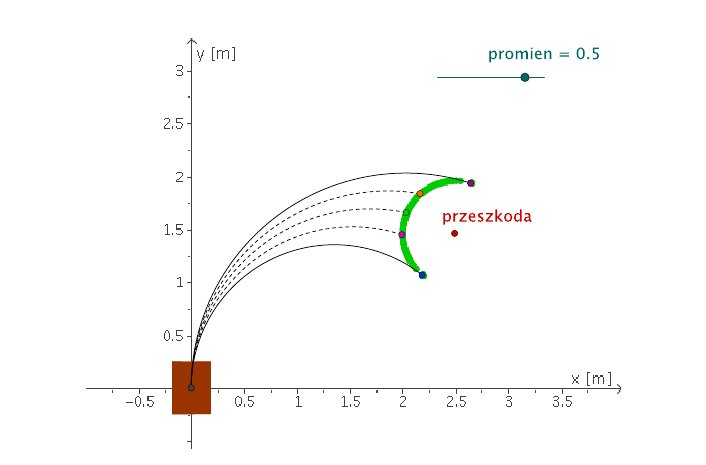
\includegraphics[scale=0.45]{./algorytmy/CVM_segmentacja}
	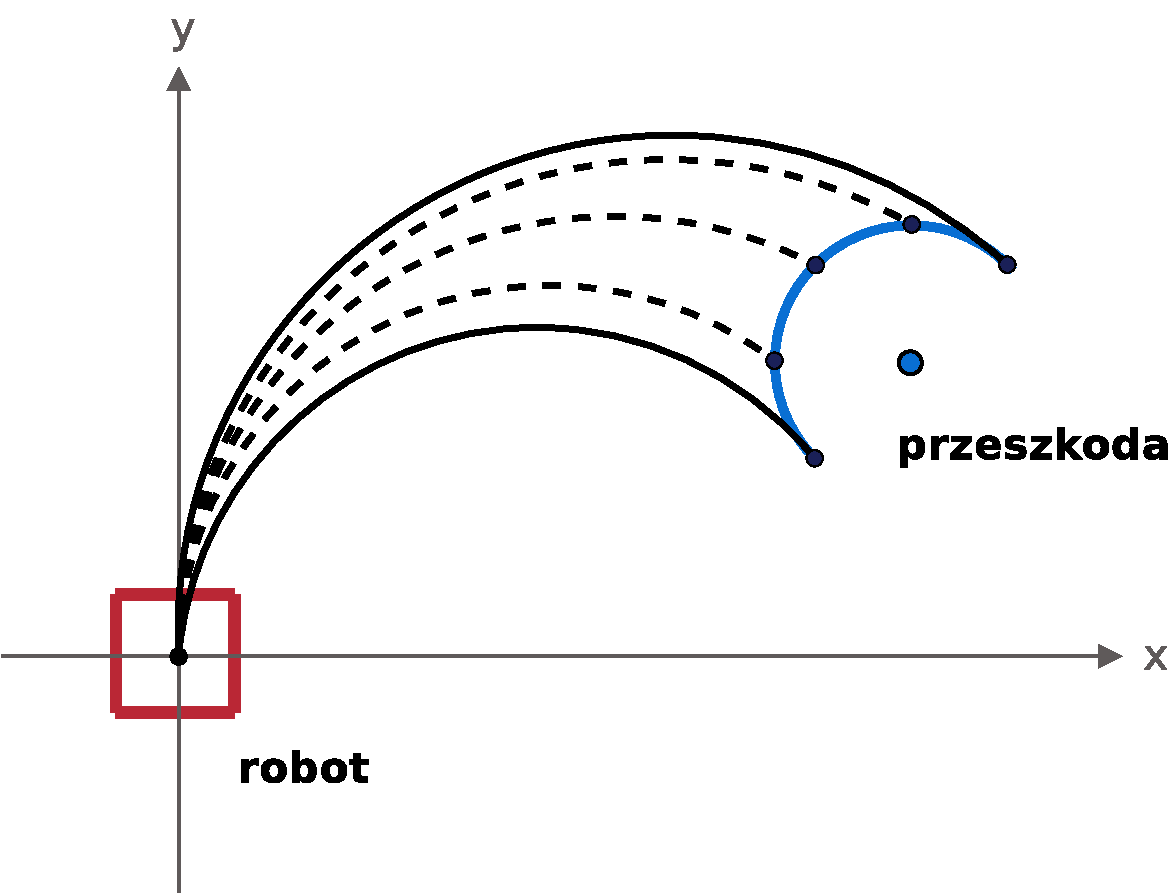
\includegraphics[scale=0.40]{./algorytmy/CVM_segmentacja_new}
	\caption{ Ukazanie sensu zastosowania segmentacji} \label{fig:CVM_segmentacja}
	\end{figure}

	Jednym z możliwych rozwiązań powyższego problemu jest podzielenie przedziału $[c_{min},c_{max}]$ na kilka
	podprzedziałów i do każdego z nich zastosowanie równania (\ref{eq:CVM_dv_const}) w celu wyznaczenia odległości od przeszkody. W pracy przyjęto rozwiązanie analogiczne jak opisane w \cite{majchrowski}.
	Pierwszym etapem jest wyznaczenie punktu leżącego na okręgu reprezentującym przeszkodę położonego najbliżej robota zgodnie z  metryką euklidesową. Następnie okrąg jest dzielony symetrycznie na $k$  segmentów. Postępowanie takie zostało przedstawione na rysunku \ref{fig:CVM_segmentacja2}. 
	Dla każdych dwóch sąsiadujących ze sobą punktów leżących pomiędzy punktami styczności $P_{min}$ oraz $P_{max}$
 	wyznaczane są krzywizny $c_1$ oraz $c_2$ i tworzony jest przedział. Jako odległość przyjmowana jest krótsza 
	z odległości zgodnie ze wzorem (\ref{eq:CVM_dv_const}). Tak otrzymane przedziały są dodawane do listy za pomocą algorytmu \ref{alg:CVM_lista}.
	
	\begin{figure}[H]
	\centering
	%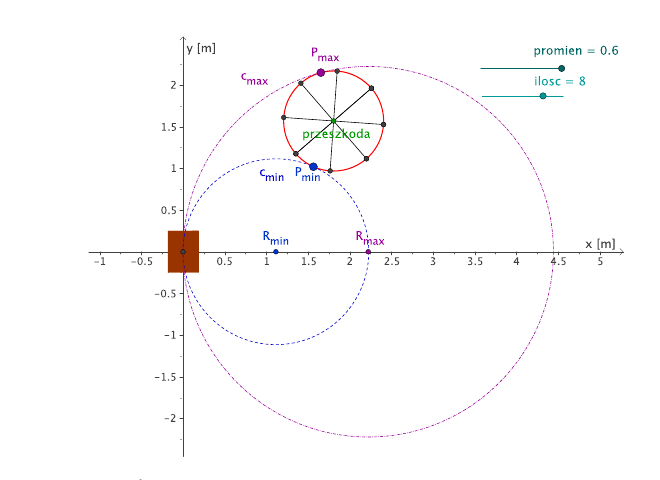
\includegraphics[scale=0.40]{./algorytmy/CVM_segmentacja2}
	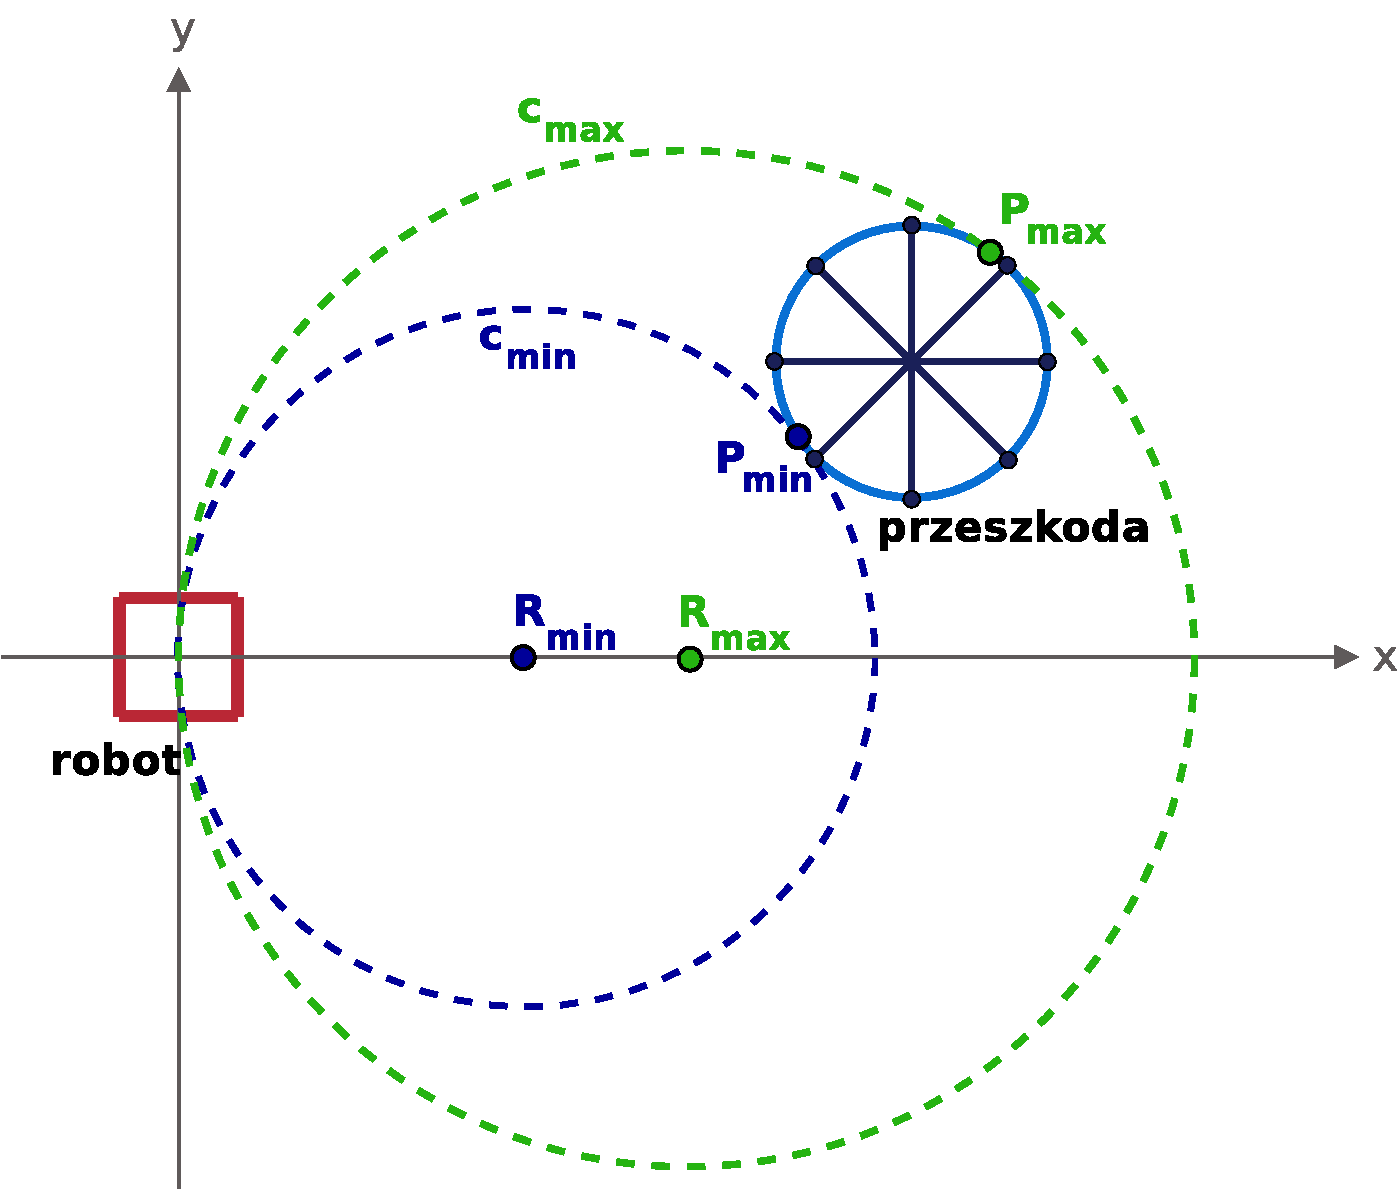
\includegraphics[scale=0.34]{./algorytmy/CVM_segmentacja2_new}
	\caption{ Efekt podziału okręgu na części} \label{fig:CVM_segmentacja2}
	\end{figure} 
\section{Algorytm RRT\\(\texttt{Rapidly-Exploring Random Tree}) \label{sec:RRT:basic}}
Kolejnym zupełnie odmiennym podejściem w planowaniu bezkolizyjnej ścieżki jest losowe przeszukiwanie dopuszczalnej przestrzeni położeń robota. Szczegółowe informacje na
jego temat można znaleźć w \cite{RRT} oraz w \cite{RRT2}.
Algorytm \texttt{RRT} jest wydajnym algorytmem, który w czasie rzeczywistym może wyznaczyć drogę do celu, jednak nie jest ona optymalna pod względem dynamiki, kinematyki ani długości.
Podstawową strukturą danych na której operuje algorytm jest drzewo. Jako korzeń przyjmowany jest stan reprezentujący położenie robota w momencie uruchomienia algorytmu.
Budowa drzewa polega na dodawaniu kolejnych węzłów do drzewa w kierunku punktu obranego w danym kroku jako docelowy. Tymczasowy stan docelowy generowany jest w następujący sposób:
 \begin{algorithm}[H]
	\caption{ Funkcja obliczająca stan docelowy }
	\label{alg:chooseTarget}
	\begin{algorithmic}
	\STATE \texttt{function} \textit{chooseTarget}(\textit{goal:state}) \textit{state};
	\STATE p = \texttt{uniformRandom in}$[0.0 ...1.0]$
	\IF{$0.0<p<goalProb$} 
	  \RETURN  \texttt{goal};
	\ELSIF{ $goalProb<p<1.0$}
	  \RETURN \textit{RandomState()}
	\ENDIF
	\end{algorithmic}
  \end{algorithm}

Na listingu \ref{alg:chooseTarget} użyta została funkcja \texttt{RandomState()} zwracająca losowy punkt ze zbioru wszystkich możliwych położeń robota.
W najprostszej realizacji może ona zwracać współrzędne punktu dobierane z rozkładem jednostajnym z zadanego przedziału.
W każdej iteracji algorytmu tymczasowy stan docelowy obliczany jest na nowo. Aktualne drzewo, na którym operuje algorytm przeszukiwane jest w celu znalezienia
węzła \texttt{nearest} znajdującego się najbliżej tego celu. Węzeł \texttt{nearest} rozszerzany jest w kierunku tegóż celu za pomocą funckji \texttt{extend}.
Operacja ta w najprostszym ujęciu polega na stworzeniu nowego węzła przesuniętego względem \texttt{nearest} o odcinek \texttt{rrtStep} w kierunku tymczasowego celu.
Istotne jest, aby sprawdzić czy nowo wygenerowany stan znajduje się w dopuszczalnej przestrzeniu stanów \textdollar. W najprostszym wariancie można zastosować
heurystykę sprawdzającą jedynie czy położenie to nie koliduje z żadną z przeszkód znajdujących się w danej sytuacji oraz czy robot jest w stanie do niego dotrzeć.
Bardziej zaawansowane heurystyki powinny sprawdzać czy na przykład podczas przemieszczania  się do nowej pozycji nie nastąpi kolizja z dynamiczną przeszkodą.
W ogólnym ujęciu algorytm \texttt{RRT} wygląda zatem następująco:
  \begin{algorithm}[H]
	\caption{ Ogólna zasada algorytmu \texttt{RRT} }
	\label{alg:RRT}
	\begin{algorithmic}
	\STATE zbuduj model eksplorowanego świata $\mapsto$ \texttt{env:environment};
	\STATE zainicjuj stan początkowy $\mapsto$ \texttt{initState:state};
	\STATE zainicjuj stan końcowy $\mapsto$ \texttt{goalState:state};
	\STATE
	\WHILE { \texttt{goalState.distance(nextState)} $>$ \texttt{minimalDistance} }
	  \STATE wybierz tymczasowy cel: \texttt{target} =  \texttt{chooseTarget(goalState)}
	  \STATE nearestState $=$ \texttt{ nearest(tree, target) }
	  \STATE \texttt{extendedState} $=$ \texttt{extend(env, nearest, target)}
	  \IF { \texttt{extendedState} $!=$ \texttt{NULL} } 
	    \STATE \texttt{addNode(tree, extended)}
	  \ENDIF
	\ENDWHILE
	\RETURN  \texttt{tree};
	\end{algorithmic}
  \end{algorithm}
W opisie algorytmu \ref{alg:RRT} użyte zostały nie omówione jeszcze funkcje, \texttt{distance} zwracająca odległość w sensie euklidesowym między dwoma węzłami drzewa,
\texttt{addNode} dodająca węzeł do bieżącego drzewa. Parametr \texttt{rrtStep} jest natomiast wyrażony w metrach.
Tak zaimplementowana wersja algorytmu może być zastosowana jako skuteczne narzędzie do bezkolizyjnej nawigacji robotem, jednak jego wydajność można poprawić poprzez
modyfikacje opisane w kolejnym podrozdziale.

\subsection{Modyfikacje algorytmu, czyli przejście z \texttt{RRT} do \texttt{ERRT} \label{sec:RRT:extend} }
Omawiany algorytm można zmodyfikować pod kątem szybkości działania. Po pierwsze elementy drzewa można przechowywać w strukturach ułatwiających przeszukiwanie drzewa,
w literaturze stosowane są w tym celu \texttt{KD-drzewa}. Kolejną modyfikacją jest zapamiętywanie losowo wybranych węzłów ze ścieżki znalezionej w poprzednim uruchomieniu
algorytmu. W takim wariancie tymczasowy punkt docelowy obierany jest następująco:
 \begin{algorithm}[H]
	\caption{ Zmodyfikowana funkcja obliczająca stan docelowy }
	\label{alg:chooseTargetExt}
	\begin{algorithmic}
	\STATE \texttt{function} \textit{chooseTargetExt}(\textit{goal:state}) \textit{state};
	\STATE p = \texttt{uniformRandom in}$[0.0 ...1.0]$
	\STATE i = \texttt{uniformRandom in}$[0 ...number\_of\_waypoints -1]$
	\IF{$0.0<p<goalProb$} 
	  \RETURN  \texttt{goal};
	\ELSIF{ $goalProb<p<goalProb+wayPointProb$}
	  \RETURN \textit{WayPoints[i]}
	\ELSIF{ $goalProb+wayPointProb<p<1.0$}
	  \RETURN \textit{RandomState()}
	\ENDIF
	\end{algorithmic}
  \end{algorithm}
W publikacji \cite{RRT} prawdopodobieństwo podążania do właściwego celu ostatecznie ustalane zostało na poziomie $0.1$, natomiast \texttt{wayPointProb} wynosiło $0.7$.


\begin{figure}[h]
\centering
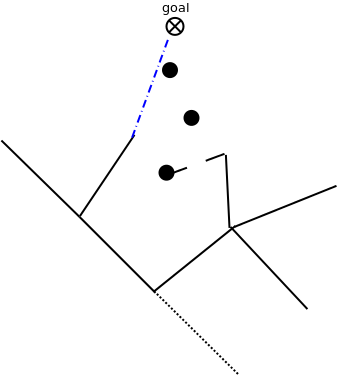
\includegraphics[scale=0.34]{./algorytmy/tree_with_waypoints.png}
\caption{ \texttt{RRT} z zapamiętanymi węzłami z porzedniego uruchomiena. Linią kropkowaną zaznaczono gałąź dodaną w kierunku losowego punktu,
 linią przerywaną w kierunku jednego z elementów z poprzedniej ścieżki, a linią niebiską w kierunku celu.} \label{fig:tree_with_waypoints}
\end{figure} 

\todo{przetłumaczyć na polski}
The distance metric can be modified to
include not only the distance from the tree to a target
state, but also the distance from the root of the
tree, multiplied by some gain value.

\section{Zalety algorytmu RRT w stosunku \\do CVM}
Podczas kontynuacji prac nad rozgrywkami RoboCup zdecydowano się na zmianę algorytmu wyznaczającego bezkolizyjną ścieżkę. Zmiana została wymuszona decyzją o zmianie
modelu sterowanego robota. Bazę jezdną o napędzie różnicowym zastąpiono holonomiczną. Algorytm \textit{CVM} jest algorytmem dedykowanym do robotów o napędzie różnicowym, doskonale
można ująć w nim ograniczenia na dopuszczalne prędkości. Jednak sterowanie za jego pomocą robotem holonomicznym nie pozwala na pełne wykorzystanie możliwości robota.
Dodatkowo jak zostało udowodnione w pracy inżynierskiej \cite{inzynierka}, \textit{CVM} w przypadku środowisk z przeszkodami dynamicznymi osiągał skuteczność na poziomie $80\%$. Kolizje występowały 
głównie w sytuacjach, kiedy przeszkoda uderzała w robota z boku lub z tyłu. Wynikało to z faktu, że trajektoria ruchu takiej przeszkody znajdowała się poniżej osi $OY$ w układzie współrzędnych
związanym ze sterowanym robotem. Przeszkody takiego typu nie były uwzględnianie przez algorytm.
\textit{RRT} pozwala na uwzględnianie przeszkód rozsianych po całej planszy. Dodatkowo umożliwia poruszanie się po bardziej złożonych trajektoriach.
Kolejną zaletą \textit{RRT} jest prostota w ograniczaniu przestrzeni z której losowane są tymczasowe punkty docelowe. Dzięki temu w prosty sposób można ograniczyć poruszanie
się robota tylko do wnętrza boiska, w przypadku \textit{CVM} istniała konieczność modelowania bandy boiska jako zbioru okręgów, mnożyło to ilość obiektów z jakimi należało detekować
kolizje.
Kolejnym problemem \textit{CVM} jest nawigacja do celu znajdującego się za robotem, w pracy inżynierskiej wprowadzono modyfikację, zmieniającą parametr odpowiedzialny za kierowanie
robota na cel, uzależniając go od orientacji robota względem celu. Intencją było wymuszenie obrotu robota w kierunku celu, w sytuacji gdy orientacja do celu jest duża.
Modyfikacja poprawiła skuteczność jednak, nawet dla najlepszego zestawu wag wynosiła ona $80\%$. W przypadku bazy holonomicznej obracanie się w kierunku punktu docelowego nie jest
konieczne, stąd takie sterowanie nie jest optymalne.

\input{./tex/opis_testy_rrt}

\input{./tex/stp}

\chapter[Podsumowanie]{Podsumowanie}
\chaptermark{Podsumowanie}
Podczas realizacji niniejszej pracy stworzono środowisko symulacyjne umożliwiające modelowanie rozgrywek robotów z ligi \emph{Small-Size League}. Ponieważ wcześniejsze prace, opisane w~\cite{inzynierka}
prowadzono na platformie Player/Stage/Gazebo, zdecydowano się na dalszą pracę z tym środowiskiem. Uaktualniono natomiast wersję stosowanego oprogramowania. Opracowano także nowe modele robotów
oraz boiska. Wykorzystywane w trakcie eksperymentów modele robotów wzorowane były na rzeczywistych zawodnikach rozgrywek RoboCup. Zmiana bazy jezdnej na wielokierunkową wymusiła implementację nowego sterownika
robota. Przygotowane środowisko, może posłużyć do dalszych prac na rozgrywkami robotów w piłkę nożną.

W ramach pracy zaimplementowano także algorytm unikania kolizji RRT. Zachowanie algorytmu sprawdzone zostało w środowiskach testowych wykorzystywanych w~\cite{inzynierka}. Dzięki takiemu podejściu
można było dokonać porównania RRT z wcześniej stosowanym CVM. W wyniku przeprowadzonych eksperymentów udowodniono, że w danych sytuacjach algorytm RRT osiąga dużo lepsze wyniki niż CVM.
Wybrana metoda rozwiązała także kilka problemów, z którymi CVM nie był w stanie sobie poradzić. Poprzednie rozwiązanie, osiągało dużo słabsze efekty w sytuacjach, kiedy cel znajdował się za robotem.
Algorytm był także mało skuteczny, gdy punkt docelowy znajdował się za zaporą utworzoną z kilku robotów. W przypadku RRT nie zauważono takich zachowań.
Sama metoda okazała się też dużo mniej wrażliwa na dobór parametrów z jakimi jest ona uruchamiana (zupełnie przeciwnie zachowywał się CVM). W przypadku silnie dynamicznego środowiska
jest to bardzo pożądana cecha. Zastosowany algorytm okazał się także szybką metodą, co ma duże znaczenie w rozgrywkach.

W dalszej części został omówiony i zaimplementowany algorytm planowania i koordynacji działań robotów wzorowany na architekturze STP opisany w \cite{stp}. W ramach pracy zrealizowano w pełni dwie
warstwy z oryginalnego rozwiązania (\texttt{skills} i \texttt{tactics}). Stworzone oporogramowanie umożliwa wykonywanie robotom podstawowych elementów gry w piłkę nożna (prowadzenie piłki, strzał na bramkę,
podanie piłki do innego zawodnika), jak i bardziej złożonych zachowań. Algorytm został przetestowany podczas realizacji wybranych zadań eliminacyjnych,
którym musieli sprostać uczestnicy rozgrywek RoboCup w ostatnich latach. W tym celu stworzono także prostą wartswę \texttt{play}, zapewniającą koordynację w obrębie drużyny
oraz opracowano plany gry rozwiązujące zadania testowe. Otrzymane wyniki zostały porównane z rezultatami uczestników mistrzostw. W przypadku pierwszego eksperymentu zaimplementowane
rozwiązanie plasowałoby się na trzecim miejscu, natomiast w przypadku drugiego eksperymentu realne byłoby miejsce drugie. Należy jednak oczywiście pamietać, że sterowanie symulowanym
robotem jest dużo prostsze niż rzeczywistym. Przeprowadzone eksperymenty potwierdzają, że podejście STP może z powodzeniem służyć do koordynacji i planowania działań podczas rzeczywistej rozgrywki.
Niewątpliwą zaletą architektury STP jest jej funkcjonalność, zachowania zawodników mogą być zmieniane na trzech poziomach w zależności od sytuacji na planszy.

Niniejsza praca dostarcza gotowe środowisko testowe wraz z aplikacją sterującą. Elementy te mogą zostać wykorzystane podczas dalszych prac nad rozgrywkami RoboCup. Stworzone oprogramowanie można
dalej rozwijać w kierunku przeprowadzenia pełnej rozgrywki wzorowanej na  \emph{Small-Size League}.

\appendix
\chapter[Zawartość płyty CD ]{Zawartość płyty CD}
\chaptermark{Zawartość płyty CD}	
Dołączona do pracy płyta CD zawiera następujące elementy:
\begin{itemize}
\item pliki źródłowe wykorzystanej wersji symulatora \textit{Gazebo} wraz z wprowadzonymi poprawkami opisanymi w par.~\ref{subsect:realizacjaROBOCUP} oraz zaimplementowanym
sterownikiem holonomicznej bazy jezdnej -- folder \texttt{gazebo},
\item opracowane modele robotów, oraz boiska  -- folder \texttt{modele},
\item kod źródłowy aplikacji opracowanej aplikacji (projekt w środowisku \mbox{Eclipse}\footnote{Środowisko jest dostępne pod adresem \url{www.eclipse.org}.} dla C++) -- folder \texttt{aplikacja\_sterujaca},
\item kod źródłowy  aplikacji \textit{RRT\_debug} służącej do wizualizacji działania algorytmu RRT -- folder \texttt{RRT\_debug}, 
\item otrzymane wyniki przeprowadzonych eksperymentów wraz ze skryptami do tworzenia wykresów -- folder \texttt{wyniki},
\item zrzuty ekranu prezentujące wykonane modele oraz filmy z symulatora pokazujące realizację przeprowadzonych eksperymentów -- folder \texttt{media},
\item plik \texttt{praca\_magisterska.pdf} -- wersja elektroniczna niniejszego dokumentu.
\end{itemize}


% \chapter[Instrukcja instalacji Gazebo]{Instrukcja instalacji Gazebo}
% \chaptermark{Instrukcja instalacji Gazebo}
% \todo{poprawic opis instalacji gazebo}
% \todo{zmienic numery rewizji zastosowanych aplikacji}
% Instrukcję instalacji można znaleźć w poradniku dostępnym pod adresem \url{http://playerstage.sourceforge.net/doc/Gazebo-manual-svn-html/install.html}. \newline
% W~razie problemów można skorzystać także z opisu dostępnego pod adresem \newline \url{http://www.irobotics.org/gazebo08.f8.html}. 
% Do instalacji należy użyć wersji \textit{Gazebo} dostępnej na płycie CD dołączonej do pracy 
% (jest to wersja 6782 dostępna poprzez repozytorium SVN, zawiera jednak poprawki opisane w~par.~\ref{subsect:realizacjaROBOCUP}).
%  Do poprawnej pracy \textit{Gazebo} wymagana jest obecność dodatkowych aplikacji. Najważniejsze z nich wykorzystano w niniejszej pracy w nastepujących wersjach:
% \begin{itemize}
%  \item Player (wymagany do kompilacji Gazebo) -- pobrany z repozytorium SVN w wersji 6350,
%  \item ODE pobrane z oficjalnego repozytorium SVN, wersja 1451,
%  \item OGRE w wersji 1.4.7,
%  \item pozostałe wymagane aplikacje zostały zainstalowane w wersjach zgodnych z opisem w podręczniku instalacji.
% \end{itemize}


%\input{./tex/dodatek_CVM}
\chapter[Szczegóły eksperymentów]{Szczegóły eksperymentów \label{sec:szczegoly_eksp}}
\chaptermark{Szczegóły eksperymentów}
Dodatek zawiera poglądowe rysunki przedstawiające środowiska testowe, na których przeprowadzane były eksperymenty.
Na każdym z nich zaznaczono inne roboty nie podlegające sterowaniu przez testowany algorytm oraz początkowe położenie 
i orientację sterowanego robota. 
W przypadku eksperymentów w środowisku dynamicznym zaznaczono także kierunek i zwrot prędkości z jaka poruszały się przeszkody.
Poniżej zamieszczono legendę objaśniającą znaczenie użytych symboli.
	\begin{figure}[H]
	\centering
	\includegraphics[scale=0.35]{./eksperymenty/srodowiska/legenda}
	\end{figure}	

W drugiej części dodatku zamieszczono tabelę z zastosowanymi podczas eksperymentów z użyciem algorytmu \textit{CVM} zestawami wag. Ponieważ każda ze składowych funkcji celu (\ref{eq:fcelu_cvm}) algorytmu  zwraca wartość z przedziału 
$[0;1]$ zdecydowano się na przetestowanie takich trójek liczb z tego przedziału,  które sumują się do jedności.
\section*{Środowiska testowe\label{sec:srodowiska_testowe}}
\subsection*{statyczne:}
	\begin{figure}[H]
	\centering	
	\subfloat[]{\includegraphics[scale=0.3]{./eksperymenty/srodowiska/eksperyment00}} 
	\hspace{0.5cm}
	\subfloat[]{\includegraphics[scale=0.3]{./eksperymenty/srodowiska/eksperyment01}}    \\
	\subfloat[]{\includegraphics[scale=0.3]{./eksperymenty/srodowiska/eksperyment05}} 
	\hspace{0.5cm}
	\subfloat[]{\includegraphics[scale=0.3]{./eksperymenty/srodowiska/eksperyment06}}  \\

	\end{figure}	

	\begin{figure}[H]
	\centering
	\subfloat[]{\includegraphics[scale=0.3]{./eksperymenty/srodowiska/eksperyment09}} 
	\hspace{0.5cm}
	\subfloat[]{\includegraphics[scale=0.3]{./eksperymenty/srodowiska/korytarz}}  	\\
	\subfloat[]{\includegraphics[scale=0.3]{./eksperymenty/srodowiska/prosta}} 
	\hspace{0.5cm}
	\subfloat[]{\includegraphics[scale=0.3]{./eksperymenty/srodowiska/waskie_przejscie}}  \\
	\end{figure}
	\begin{figure}[H]
	\centering
	\subfloat[]{\includegraphics[scale=0.3]{./eksperymenty/srodowiska/atak1}} 
	\hspace{0.5cm}
	\subfloat[]{\includegraphics[scale=0.3]{./eksperymenty/srodowiska/atak2}}
	\end{figure}
\subsection*{dynamiczne:}
	\begin{figure}[H]
	\centering
	\subfloat[]{\includegraphics[scale=0.3]{./eksperymenty/srodowiska/dynamiczne/eks01}} 
	\hspace{0.5cm}
	\subfloat[]{\includegraphics[scale=0.3]{./eksperymenty/srodowiska/dynamiczne/eks02}}    \\
	\end{figure}
	\begin{figure}[H]
	\centering
	\subfloat[]{\includegraphics[scale=0.3]{./eksperymenty/srodowiska/dynamiczne/eks03}} 
	\hspace{0.5cm}
	\subfloat[]{\includegraphics[scale=0.3]{./eksperymenty/srodowiska/dynamiczne/eks04}}  \\
	\subfloat[]{\includegraphics[scale=0.3]{./eksperymenty/srodowiska/dynamiczne/eks05}} 
	\hspace{0.5cm}
	\subfloat[]{\includegraphics[scale=0.3]{./eksperymenty/srodowiska/dynamiczne/eks06}}  	\\
	\end{figure}	
	\begin{figure}[H]
	\centering
	\subfloat[]{\includegraphics[scale=0.3]{./eksperymenty/srodowiska/dynamiczne/eks07}} 
	\hspace{0.5cm}
	\subfloat[]{\includegraphics[scale=0.3]{./eksperymenty/srodowiska/dynamiczne/eks08}}  \\
	\subfloat[]{\includegraphics[scale=0.3]{./eksperymenty/srodowiska/dynamiczne/eks09}} 
	\hspace{0.5cm}
	\subfloat[]{\includegraphics[scale=0.3]{./eksperymenty/srodowiska/dynamiczne/eks10}}
	\end{figure}	

\section*{Zestawy wag używane w eksperymentach \label{sec:zestawy_wag}}
\begin{table}[H]
\centering
\scalebox{0.8}{
\begin{tabular}[t]{|c ||c |c| }
\hline
Zestaw wag & $goalProb$ & $wayPointProb$ \\ \hline\hline
1 & 0.0 & 0.0\\ \hline
2 & 0.0 & 0.2\\ \hline
3 & 0.0 & 0.3\\ \hline
4 & 0.0 & 0.4\\ \hline
5 & 0.0 & 0.5\\ \hline
6 & 0.0 & 0.6\\ \hline
7 & 0.0 & 0.7\\ \hline
8 & 0.0 & 0.8\\ \hline
9 & 0.0 & 0.9\\ \hline
10 & 0.0 & 1.0\\ \hline
11 & 0.1 & 0.0\\ \hline
12 & 0.1 & 0.1\\ \hline
13 & 0.1 & 0.2\\ \hline
14 & 0.1 & 0.3\\ \hline
15 & 0.1 & 0.4\\ \hline
16 & 0.1 & 0.5\\ \hline
17 & 0.1 & 0.6\\ \hline
18 & 0.1 & 0.7\\ \hline
19 & 0.1 & 0.8\\ \hline
20 & 0.1 & 0.9\\ \hline
21 & 0.2 & 0.0\\ \hline
22 & 0.2 & 0.1\\ \hline
23 & 0.2 & 0.2\\ \hline
24 & 0.2 & 0.3\\ \hline
25 & 0.2 & 0.4\\ \hline
26 & 0.2 & 0.5\\ \hline
27 & 0.2 & 0.6\\ \hline
28 & 0.2 & 0.7\\ \hline
29 & 0.2 & 0.8 \\ \hline
30 & 0.3 & 0.0 \\ \hline
31 & 0.3 & 0.1 \\ \hline
32 & 0.3 & 0.2 \\ \hline
33 & 0.3 & 0.3 \\ \hline
\end{tabular}
}
\hspace{0.5cm}
\scalebox{0.8}{
\begin{tabular}[t]{|c ||c |c| }
\hline
Zestaw wag &$goalProb$ & $wayPointProb$\\ \hline\hline
34 & 0.3 & 0.4 \\ \hline
35 & 0.3 & 0.5 \\ \hline
36 & 0.3 & 0.6 \\ \hline
37 & 0.3 & 0.7 \\ \hline
38 & 0.4 & 0.0 \\ \hline
39 & 0.4 & 0.1 \\ \hline
40 & 0.4 & 0.2 \\ \hline
41 & 0.4 & 0.3 \\ \hline
42 & 0.4 & 0.4 \\ \hline
43 & 0.4 & 0.5 \\ \hline
44 & 0.4 & 0.6 \\ \hline
45 & 0.5 & 0.0 \\ \hline
46 & 0.5 & 0.1 \\ \hline
47 & 0.5 & 0.2 \\ \hline
48 & 0.5 & 0.3 \\ \hline
49 & 0.5 & 0.4 \\ \hline
50 & 0.5 & 0.5 \\ \hline
51 & 0.6 & 0.1 \\ \hline
52 & 0.6 & 0.2 \\ \hline
53 & 0.6 & 0.3 \\ \hline
54 & 0.6 & 0.4 \\ \hline
55 & 0.7 & 0.0 \\ \hline
56 & 0.7 & 0.1 \\ \hline
57 & 0.7 & 0.2 \\ \hline
58 & 0.7 & 0.3 \\ \hline
59 & 0.8 & 0.0 \\ \hline
60 & 0.8 & 0.1 \\ \hline
61 & 0.8 & 0.2 \\ \hline
62 & 0.8 & 0.2 \\ \hline
63 & 0.9 & 0.0 \\ \hline
64 & 0.9 & 0.1 \\ \hline
65 & 1.0 & 0.0 \\ \hline
\end{tabular}
}
\end{table}



\begin{thebibliography}{9}
\bibitem{robocup}
	Oficjalna strona Ligi \textit{RoboCup} dostępna pod adresem:\\
	\url{www.robocup.org}
	
\bibitem{RRT}
J. Bruce, M. Veloso:
\emph{Real-Time Randomized Path Planning for Robot Navigation}. Carnegie Mellon University

\bibitem{RRT2}
J.Kim J.M. Esposito, V. Kumar:
\emph{An RRT-Based algorithm for testing and validating multi-robot controllers}. University of Pennsylvania, US Naval Academy

\bibitem{duleba}
	I. Dulęba:
	\emph{Metody i algorytmy planowania ruchu robotów mobilnych i manipulacyjnych}.
	Warszawa, Akademicka Oficyna Wydawnicza EXIT, 2001.

\bibitem{CVM_1}
	T. Quasn, L.Pyeatt, J.Moore:
	\emph{Curvature-Velocity Method for Differentially Steered Robots}.
	AI Robotics Lab
	Computer Science Department,
	Texas Tech University, 2003.

\bibitem{CVM_2}
	R. Simmons:
	\emph{The Curvature-Velocity Method for Local Obstacle Avoidance}.
	School of Computer Science,
	Carnegie Mellon University, 1996.
\bibitem{majchrowski}
	M. Majchrowski:
	\emph{Algorytm unikania kolizji przez robota mobilnego bazujący na przeszukiwaniu
	przestrzeni prędkości}.
	Praca Magisterska, Politechnika Warszawska, 2006.

\bibitem{VFH_1}
	J. Borenstein, Y. Koren:
	\emph{ The vector field histogram -- fast obstacle avoidance for mobile robots}.
	IEEE Transaction on Robotics and Automation, 1991.

\bibitem{VFH_2}
	J. Borenstein,Y. Koren:
	\emph{Histogramic in-motion mapping
	for mobile robot obstacle avoidance}.
	Department of Mechanical Engineering and Applied Mechanics,
	The University of Michigan, 1991.

\bibitem{dynamic_window}
	D. Fox, W. Burgard, S. Thrun:
	\emph{The Dynamic Window Approach to Collision Avoidance}.
	Department of Computer Science, University of Bonn;
	Department of Computer Science, Carnegie Mellon University, Pittsburgh, 1991.
		
 \bibitem{stp}
	B.Browning, J.Bruce, M.Bowling, M.Veloso:
	\emph{STP: Skills, tactics and plays for multi-robot control
             in adversarial environments.}
	  Carnegie Mellon University, Pittsburgh. 2004.

 \bibitem{omni_base_1}
	R.Rojas, A.Gloye F\"{o}orster:
	\emph{ Holonomic Control of a robot with an omnidirectional
	      drive. }
	  Freie Universität Berlin, 2006.

\bibitem{omni_base_2}
	R.Rojas, A.Gloye F\"{o}orster:
	\emph{ Design of an omnidirectional universal mobile platform. }
	  Eindhoven University of Technology, 2005.	  
\bibitem{inzynierka}
	M.Gąbka, K.Muszyński
	Praca dyplomowa inzynierska
	\emph{Środowisko symulacyjne i algorytm unikania kolizji robota mobilnego
	grającego w piłkę nożną}
	Politechnika Warszawska, 2008.

\bibitem{trapezy1}
	J.Bruce, M.Bowling, B.Browning, M.Veloso
	\emph{Multi-Robot Team Response to a Multi-Robot Opponent Team}
	Carnegie Mellon University, Pittsburgh.

\bibitem{trapezy2}
	J.Bruce, M.Veloso
	\emph{Real-time multi-robot motion planning with safe dynamics}
	Carnegie Mellon University, Pittsburgh.

\bibitem{navi_func1}
	D. E. Koditschek, and E.Rimon 
	\emph{ Robot navigation functions on manifolds with boundary }
	Advances in Applied Mathematics
	Volume 11 Issue 4, Dec. 1990.

\bibitem{navi_func2}
	D. E. Koditschek, and E.Rimon 
	\emph{Exact robot navigation using artificial potential functions }
	IEEE Transactions on Robotics and Automation.
	Vol. 8, no. 5, pp. 501-518. Oct. 1992
\bibitem{ISR}
	C. Zieliński, W. Szynkiewicz:
	\emph{Konspekt do wykładu: Inteligentne Systemy robotyczne}.
	Politechnika Warszawska, 2008.
\bibitem{gazebo_experts}
	N. Koenig:
	\emph{Gazebo. The Instant Expert's Guide}.
	Player Summer School on Cognitive Robotics, Monachium 2007.
\bibitem{hamada_mgr}
 M.Hamada
 \emph{Układ sterowania autonomicznym robotem mobilnym}. Praca magisterska, Politechnika Warszawska, 2007.
\end{thebibliography}



\end{document}